\newpage
\section{TỔNG VÀ HIỆU CỦA HAI VECTƠ}
\subsection{LÝ THUYẾT CẦN NHỚ}
\subsubsection{Tổng của hai vectơ}
\indam{Định nghĩa:}
\begin{boxdn}
Cho hai vectơ $\overrightarrow{a}$ và $\overrightarrow{b}$. Từ một điểm $A$ tuỳ ý, lấy hai điểm $B$, $C$ sao cho $\overrightarrow{AB}=\overrightarrow{a}$, $\overrightarrow{BC}=\overrightarrow{b}$. Khi đó $\overrightarrow{AC}$ được gọi là tổng của hai vectơ $\overrightarrow{a}$, $\overrightarrow{b}$ và được kí hiệu là $\overrightarrow{a}+\overrightarrow{b}$.
\begin{center}
	\begin{tikzpicture}[scale=1, line join=round, line cap=round, >=stealth]
	%% Khai bao diem
	\def\d{6} \def\r{4}
	\foreach \x in {0,1,2,...,\r}
	{\draw[dashed,gray!40] (0,\x)--(\d,\x);}
	\foreach \x in {0,1,2,...,\d}
	{\draw[dashed,gray!40] (\x,0)--(\x,\r);}
	\path
	(0,2) coordinate (X)
	(1,0) coordinate (Y)
	(1,3) coordinate (A)
	(2,1) coordinate (B)
	(3,0) coordinate (Z)
	(6,2) coordinate (T)
	(5,3) coordinate (C)
	;
	
	\draw[thick,-{Stealth[length=2.5mm]}] (X)--(Y);
	\draw[thick,-{Stealth[length=2.5mm]}] (A)--(B);
	\draw[thick,-{Stealth[length=2.5mm]}] (Z)--(T);
	\draw[thick,-{Stealth[length=2.5mm]}] (B)--(C);
	\draw[thick,-{Stealth[length=2.5mm]},color=red] (A)--(C);
	\draw 
	($(X)!1/2!(Y)$) node [shift=(190:0.3)] {$\overrightarrow{a}$}
	($(A)!1/2!(B)$) node [shift=(190:0.3)] {$\overrightarrow{a}$}
	($(T)!1/2!(Z)$) node [shift=(-60:0.3)] {$\overrightarrow{b}$}
	($(B)!1/2!(C)$) node [shift=(-60:0.3)] {$\overrightarrow{b}$}
	($(A)!1/2!(C)$) node [shift=(90:0.3)] {$\overrightarrow{a}+\overrightarrow{b}$}
	;
	
	%% vẽ điểm
	\foreach \x/\g in {A/90,B/-90,C/90}
	\draw[fill=black] (\x) circle (.039)+(\g:.31)
	node{$\x$};	
	
\end{tikzpicture}
\end{center}
Như vậy $\overrightarrow{a}+\overrightarrow{b}=\overrightarrow{A B}+\overrightarrow{B C}=\overrightarrow{A C}$.
\end{boxdn}

\indam{Các quy tắc cộng hai vectơ}
\begin{boxdn}
\begin{itemize}
	\item \textbf{Quy tắc ba điểm.} Với ba điểm $A$, $B$, $C$ ta có $\overrightarrow{AB}+\overrightarrow{BC}= \overrightarrow{AC}$.	
	\item \textbf{Quy tắc hình bình hành.} Với $HIKL$ là hình bình hành ta có $\overrightarrow{HI}+\overrightarrow{HL}= \overrightarrow{HK}$.	
\end{itemize}

\begin{center}
	\begin{tikzpicture}[scale=1, line join=round, line cap=round, >=stealth]
		%% Khai bao diem
		\def\d{11} \def\r{4}
		\foreach \x in {0,1,2,...,\r}
		{\draw[dashed,gray!40] (0,\x)--(\d,\x);}
		\foreach \x in {0,1,2,...,\d}
		{\draw[dashed,gray!40] (\x,0)--(\x,\r);}
		\path
		(0,2) coordinate (X)
		(1,0) coordinate (Y)
		(1,3) coordinate (A)
		(2,1) coordinate (B)
		(3,0) coordinate (Z)
		(6,2) coordinate (T)
		(5,3) coordinate (C)
		(6,1) coordinate (H)
		(9,1) coordinate (I)
		(7,3) coordinate (L)
		($(I)+(L)-(H)$) coordinate (K)
		;
		
	
		\draw[thick,-{Stealth[length=2.5mm]}] (A)--(B);
		\draw[thick,-{Stealth[length=2.5mm]}] (B)--(C);
		\draw[thick,-{Stealth[length=2.5mm]},color=red] (A)--(C);
		\draw[thick,-{Stealth[length=2.5mm]}] (H)--(I);
		\draw[thick,-{Stealth[length=2.5mm]}] (H)--(L);
		\draw[thick,-{Stealth[length=2.5mm]},color=red] (H)--(K);
		\draw (H)--(I)--(K)--(L)--cycle;
		%% vẽ điểm
		\foreach \x/\g in {A/90,B/-90,C/90,H/-90,I/-90,K/90,L/90}
		\draw[fill=black] (\x) circle (.039)+(\g:.31)
		node{$\x$};	
		
	\end{tikzpicture}
\end{center}
\end{boxdn}

\indam{Các tính chất của phép cộng hai vectơ}
\begin{boxdn}
	\begin{itemize}
		\item \textbf{Tính chất giao hoán.} $\overrightarrow{a}+\overrightarrow{b}= \overrightarrow{b}+\overrightarrow{a}$.	
		\item \textbf{Tính chất kết hợp.} $\left(\overrightarrow{a}+\overrightarrow{b}\right)+\overrightarrow{c}=\overrightarrow{a}+\left(\overrightarrow{b}+\overrightarrow{c}\right)$.
		\item Với mọi vectơ $\overrightarrow{a}$ ta có $\overrightarrow{a}+\overrightarrow{0}=\overrightarrow{0}+\overrightarrow{a}=\overrightarrow{a}$.
	\end{itemize}
\end{boxdn}

\subsubsection{Hiệu hai vectơ}

\indam{Nhắc lại về hai vectơ đối nhau}
\begin{boxdn}
	\begin{itemize}
		\item Vectơ có cùng độ dài và ngược hướng với $\overrightarrow{a}$ được gọi là vectơ đối của $\overrightarrow{a}$, kí hiệu là $-\overrightarrow{a}$. 
		\item Hai vectơ $\overrightarrow{a}$ và $\overrightarrow{b}$ được gọi là đối nhau nếu chúng ngược hướng và có cùng độ dài. Khi đó $\overrightarrow{a}+\overrightarrow{b}=\overrightarrow{0}$.
	\end{itemize}
\end{boxdn}

\indam{Hiệu hai vectơ}
\begin{boxdn}
Cho hai vectơ $\overrightarrow{a}$ và $\overrightarrow{b}$. Hiệu của hai vectơ $\overrightarrow{a}$ và $\overrightarrow{b}$ là vectơ $\overrightarrow{a}+\left(-\overrightarrow{b}\right)$ và kí hiệu $\overrightarrow{a}-\overrightarrow{b}$.
\begin{center}
	\begin{tikzpicture}[scale=1, line join=round, line cap=round, >=stealth]
		%% Khai bao diem
		\def\d{6} \def\r{4}
		\foreach \x in {0,1,2,...,\r}
		{\draw[dashed,gray!40] (0,\x)--(\d,\x);}
		\foreach \x in {0,1,2,...,\d}
		{\draw[dashed,gray!40] (\x,0)--(\x,\r);}
		\path
		(0,2) coordinate (X)
		(1,0) coordinate (Y)
		(1,3) coordinate (A)
		(2,1) coordinate (B)
		(2,0) coordinate (Z)
		(6,0) coordinate (T)
		(5,3) coordinate (C)
		;
		
		\draw[thick,-{Stealth[length=2.5mm]}] (X)--(Y);
		\draw[thick,-{Stealth[length=2.5mm]}] (A)--(B);
		\draw[thick,-{Stealth[length=2.5mm]}] (Z)--(T);
		\draw[thick,-{Stealth[length=2.5mm]},color=red] (C)--(B);
		\draw[thick,-{Stealth[length=2.5mm]}] (A)--(C);
		\draw 
		($(X)!1/2!(Y)$) node [shift=(190:0.3)] {$\overrightarrow{a}$}
		($(A)!1/2!(B)$) node [shift=(190:0.3)] {$\overrightarrow{a}$}
		($(T)!1/2!(Z)$) node [shift=(-60:0.3)] {$\overrightarrow{b}$}
		($(B)!1/2!(C)$) node [shift=(-60:0.4)] {$\overrightarrow{a}-\overrightarrow{b}$}
		($(A)!1/2!(C)$) node [shift=(90:0.3)] {$\overrightarrow{b}$}
		;
		
		%% vẽ điểm
		\foreach \x/\g in {A/90,B/-90,C/90}
		\draw[fill=black] (\x) circle (.039)+(\g:.31)
		node{$\x$};	
		
	\end{tikzpicture}
\end{center}
Như vậy ta cũng có quy tắc trừ hai vectơ là: với ba điểm $A$, $B$, $C$ ta có $\overrightarrow{AB}-\overrightarrow{AC}=\overrightarrow{CB}$.\\[0.2cm]
Ta dùng quy tắc này để chèn điểm $A$ vào vectơ $\overrightarrow{CB}$.
\end{boxdn}

\indam{Tính chất vectơ của trung điểm đoạn thẳng, trọng tâm tam giác}
\begin{boxdn}
	\begin{itemize}
		\item Với $M$ là trung điểm của đoạn $AB$, ta có $\overrightarrow{MA}+\overrightarrow{MB}=\overrightarrow{0}$.	
		\item Với $G$ là trọng tâm của $\triangle ABC$, ta có $\overrightarrow{GA}+\overrightarrow{GB}+\overrightarrow{GC}=\overrightarrow{0}$.	
	\end{itemize}
\end{boxdn}

%-------------------------------------------------------------------------------------------------------------
\subsection{PHÂN LOẠI VÀ PHƯƠNG PHÁP GIẢI TOÁN}
\begin{dang}{Thực hiện phép toán cộng, trừ hai vectơ}
	\begin{itemize}
		\item [\iconMT] Nếu hai vectơ được sắp xếp thỏa mãn một trong các quy tắc (ba điểm, hình bình hành, vectơ đối) thì ta tiến hành phép cộng theo quy tắc tương ứng.
		\item [\iconMT] Nếu hai vectơ được sắp xếp chưa thỏa mãn quy tắc (điểm chưa liên tiếp, chưa cùng gốc) thì ta tiến hành dời;
		\begin{itemize}
			\item Đề không cho hình vẽ (điểm bất kì), ta dùng quy tắc 3 điểm để chèn điểm vào.
			\item Đề cho hình vẽ (tam giác, hình bình hành,...), ta dùng vectơ bằng nhau, thay vectơ này bởi vectơ khác bằng với nó sao cho có thể ghép được "quy tắc cộng" với các vectơ còn lại.
		\end{itemize}
	\end{itemize}
\end{dang}
\setcounter{vd}{0}
\begin{vd}%[Dự án đề cương 3 Khối NH24-25-Dot1-Bùi Quang Phú]%[0H5H2-1]
\immini{Cho tam giác $ABC$. Các điểm $M$, $N$ và $K$ lần lượt là trung điểm của $AB$, $AC$ và $BC$.
\begin{listEX}[1]
\item Tìm các vectơ bằng với $\overrightarrow{MK}$.
\item Tìm các vectơ đối của $\overrightarrow{MN}$.
\item Xác định các vectơ\\ $\overrightarrow{AM}+\overrightarrow{MN}$; $\overrightarrow{AM}+\overrightarrow{NK}$;  $\overrightarrow{AM}+\overrightarrow{KN}$; $\overrightarrow{AM}-\overrightarrow{AN}$; $\overrightarrow{MN}-\overrightarrow{NC}$;  $\overrightarrow{BK}-\overrightarrow{CK}$.
\end{listEX}}{
\begin{tikzpicture}[scale=1, line join=round, line cap=round]
	% Định nghĩa các điểm chính
	\coordinate (A) at (0,0);
	\coordinate (B) at (1,2);
	\coordinate (C) at (4,0);
	\foreach \p/\q/\r in {A/B/M, A/C/N, B/C/K} {
	\coordinate (\r) at ($(\p)!0.5!(\q)$);}
	\draw (A) -- (B) -- (C) -- cycle;
	\foreach \p/\pos/\lab in {A/below/A,B/above/B,C/below/C,M/above left/M,	N/below/N,K/above right/K} {
	\fill[black] (\p) circle (1pt) node[\pos, font=\footnotesize] {$\lab$};}
	\end{tikzpicture}}
\loigiai{
\begin{listEX}[1]
\item 
Vì $M$, $K$ lần lượt là trung điểm của $AB$ và $BC$ nên $MK$ là đường trung bình của $\triangle ABC$ nên $MK \parallel AC$ và $MK=AN=NC=\dfrac{1}{2}AC$
\[\overrightarrow{MK} = \overrightarrow{AN} = \overrightarrow{NC}\]
\item 
$MN$ là đường trung bình của $\triangle ABC$ nên $MN \parallel BC$ và $MN=KB=CK=\dfrac{1}{2}BC$
\[\overrightarrow{MN} = -\overrightarrow{CK} \,\,\text{và}\,\, \overrightarrow{MN}= -\overrightarrow{KB}\]
\item 
\begin{itemize}[itemsep=0.3cm]
	\item $\overrightarrow{AM} + \overrightarrow{MN} = \overrightarrow{AN}$
	\item $\overrightarrow{AM} + \overrightarrow{NK} = \overrightarrow{AM} + \overrightarrow{MB} = \overrightarrow{AB}$ \quad (vì $\overrightarrow{NK} = \overrightarrow{MB}$)
	\item $\overrightarrow{AM} + \overrightarrow{KN} = \overrightarrow{AM} + \overrightarrow{BM} = \overrightarrow{0}$ \quad (vectơ đối nhau)
	\item $\overrightarrow{AM} - \overrightarrow{AN} = \overrightarrow{NM}$
	\item $\overrightarrow{MN} - \overrightarrow{NC} = \overrightarrow{MN} + \overrightarrow{CN} = \overrightarrow{CM}$
	\item $\overrightarrow{BK} - \overrightarrow{CK} = \overrightarrow{BK} + \overrightarrow{KC} = \overrightarrow{BC}$
\end{itemize}
\end{listEX}
}
\end{vd}
%%%%=================
\begin{vd}%[Dự án đề cương 3 Khối NH24-25-Dot1-Bùi Quang Phú]%[0H5H2-1]
	\immini{Cho hình bình hành $ABCD$ tâm $O$. 
		\begin{listEX}[1]
			\item Tìm  vectơ bằng với $\overrightarrow{OC}$.
			\item Xác định các vectơ\\ $\overrightarrow{OA}+\overrightarrow{OC}$; $\overrightarrow{OB}+\overrightarrow{OD}$; $\overrightarrow{AB}+\overrightarrow{CD}$; $\overrightarrow{AD}-\overrightarrow{BC}$; $\overrightarrow{OA}+\overrightarrow{DC}$.
		\end{listEX}
	}{
		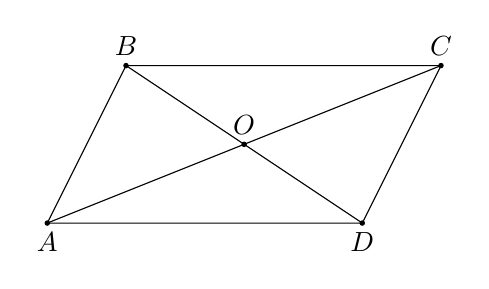
\begin{tikzpicture}[scale=1, line join=round, line cap=round]
			\coordinate (A) at (0,0);    \coordinate (B) at (1,2);
			\coordinate (C) at (5,2);    \coordinate (D) at (4,0);
			\draw (A) -- (B) -- (C) -- (D) -- cycle;
			\draw (A) -- (C) (B) -- (D);
			\coordinate (O) at (intersection of A--C and B--D);
			
			% Vẽ và gán nhãn các điểm
			\foreach \p/\pos/\lab in {
				A/below/A, B/above/B,
				C/above/C, D/below/D,
				O/above/O
			} \fill (\p) circle (1pt) node[\pos] {$\lab$};
			\end{tikzpicture}}
\loigiai{
\begin{listEX}[1]
	\item 
	Vì $O$ là tâm hình bình hành nên $\overrightarrow{OC} = \overrightarrow{AO}$.
	\item 
	\begin{itemize}[itemsep=0.3cm]
		\item $\overrightarrow{OA} + \overrightarrow{OC} = \overrightarrow{OA} + \overrightarrow{AO} = \overrightarrow{0}$;
		\item $\overrightarrow{OB} + \overrightarrow{OD} = \overrightarrow{OB} + \overrightarrow{BO} = \overrightarrow{0}$ \quad (do $\overrightarrow{OD} = \overrightarrow{BO}$);
		\item $\overrightarrow{AB} + \overrightarrow{CD} = \overrightarrow{AB} + \overrightarrow{BA} = \overrightarrow{0}$ \quad (vì $\overrightarrow{CD} = \overrightarrow{BA}$);
		\item $\overrightarrow{AD} - \overrightarrow{BC} = \overrightarrow{AD} - \overrightarrow{AD} = \overrightarrow{0}$ \quad (vì $\overrightarrow{BC} = \overrightarrow{AD}$);
		\item $\overrightarrow{OA} + \overrightarrow{DC} = \overrightarrow{OA} + \overrightarrow{AB} = \overrightarrow{OB}$.
	\end{itemize}
\end{listEX}
}
\end{vd}

\begin{dang}{Chứng minh đẳng thức vectơ}
	\begin{itemize}
		\item [\iconMT] Biến đổi từ biểu thức vế này sang vế kia.
		\item [\iconMT] Giả sử điều cần chứng minh là đúng. Ta biến đổi về điều đúng hiển nhiên.
		\item [\iconMT]Chứng minh hai biểu thức vectơ cùng bằng một biểu thức vectơ trung gian bằng cách sử dụng quy tắc trừ với điểm đầu là điểm $O$ bất kì.
	\end{itemize}
\end{dang}
\setcounter{vd}{0}
\begin{vd}%[Dự án đề cương 3 Khối NH24-25-Dot1-Bùi Quang Phú]%[0H5H2-2]
	Cho các điểm $A$, $B$, $C$, $D$, $E$, $F$. Chứng minh rằng
	\begin{listEX}[2]
		\item $\overrightarrow{AB}+\overrightarrow{CD}+\overrightarrow{EA}=\overrightarrow{CB}+\overrightarrow{ED}$; 
		\item $\overrightarrow{AD}+\overrightarrow{BE}+\overrightarrow{CF}=\overrightarrow{AE}+\overrightarrow{BF}+\overrightarrow{CD}$;
		\item $\overrightarrow{AC}+\overrightarrow{DE}-\overrightarrow{DC}-\overrightarrow{CE}+\overrightarrow{CB}=\overrightarrow{AB}$; 
		\item	$\overrightarrow{AB}-\overrightarrow{AF}+\overrightarrow{CD}-\overrightarrow{CB}+\overrightarrow{EF}-\overrightarrow{ED}=\overrightarrow{0}$.
	\end{listEX}
\loigiai{
\begin{listEX}
\item \begin{align*}
	\overrightarrow{AB} + \overrightarrow{CD} + \overrightarrow{EA} 
	&= (\overrightarrow{EA} + \overrightarrow{AB}) + \overrightarrow{CD} \\
	&= \overrightarrow{EB} + \overrightarrow{CD} \\
	&= (\overrightarrow{ED} + \overrightarrow{DB}) + (\overrightarrow{CB} + \overrightarrow{BD}) \\
	&= \overrightarrow{ED} + \overrightarrow{CB} + (\overrightarrow{DB} + \overrightarrow{BD}) \\
	&= \overrightarrow{CB} + \overrightarrow{ED}.
\end{align*}
\item \begin{align*}
	\overrightarrow{AD} + \overrightarrow{BE} + \overrightarrow{CF}
	&= (\overrightarrow{AE} + \overrightarrow{ED}) + (\overrightarrow{BF} + \overrightarrow{FE}) + (\overrightarrow{CD} + \overrightarrow{DF}) \\
	&= \overrightarrow{AE} + \overrightarrow{BF} + \overrightarrow{CD} + (\overrightarrow{ED} + \overrightarrow{FE} + \overrightarrow{DF}) \\
	&= \overrightarrow{AE} + \overrightarrow{BF} + \overrightarrow{CD}.
\end{align*}
\item  \begin{align*}
	\overrightarrow{AC} + \overrightarrow{DE} - \overrightarrow{DC} - \overrightarrow{CE} + \overrightarrow{CB} \\
	&= \overrightarrow{AC} + \overrightarrow{CB} + (\overrightarrow{DE} - \overrightarrow{DC}) - \overrightarrow{CE} \\
	&= \overrightarrow{AB} + \overrightarrow{CE} - \overrightarrow{CE} \\
	&= \overrightarrow{AB}
\end{align*}
\item \begin{align*}
	\overrightarrow{AB} - \overrightarrow{AF} + \overrightarrow{CD} - \overrightarrow{CB} + \overrightarrow{EF} - \overrightarrow{ED} \\
	&= (\overrightarrow{AB} - \overrightarrow{AF}) + (\overrightarrow{CD} - \overrightarrow{CB}) + (\overrightarrow{EF} - \overrightarrow{ED}) \\
	&= \overrightarrow{FB} + \overrightarrow{BD} + \overrightarrow{DF} \\
	&= \overrightarrow{FD} + \overrightarrow{DF} \\
	&= \overrightarrow{0}
\end{align*}
	
\end{listEX}
}
\end{vd}

\begin{vd}%[Dự án đề cương 3 Khối NH24-25-Dot1-Bùi Quang Phú]%[0H5H2-2]
	Cho tam giác $ABC$. Vẽ về phía ngoài tam giác $ABC$ các hình bình hành $ABEF$, $ACPQ$, $BCIJ$. Chứng minh $\overrightarrow{EJ}+\overrightarrow{IP}+\overrightarrow{QF}=\overrightarrow{0}$.
\loigiai{
	\begin{center}
		\begin{tikzpicture}[scale=1, line join=round, line cap=round]
		\coordinate (A) at (0,0);
		\coordinate (B) at (3,0);
		\coordinate (C) at (1.5,2);
		\coordinate (F) at ($(A)+(0.7,-1)$);
		\coordinate (E) at ($(B)+(F)-(A)$);
		\coordinate (Q) at ($(A)+(-1.2,1.5)$);
		\coordinate (P) at ($(C)+(Q)-(A)$);
		\coordinate (J) at ($(B)+(1.2,1.8)$);
		\coordinate (I) at ($(C)+(J)-(B)$);
		\draw (A) -- (B) -- (C) -- cycle;
		\draw (A) -- (F) -- (E) -- (B) -- cycle; % ABEF
		\draw (A) -- (Q) -- (P) -- (C) -- cycle; % ACPQ
		\draw (B) -- (J) -- (I) -- (C) -- cycle; % BCIJ
		\foreach \p/\pos/\lab in {
			A/left/A, B/right/B, C/above/C,
			F/below left/F, E/below right/E,
			Q/above left/Q, P/above right/P,
			J/right/J, I/right/I
		} \fill (\p) circle (1pt) node[\pos] {$\lab$};
		\end{tikzpicture}
	\end{center}
	Ta có thể biểu diễn các vectơ như sau:
	\begin{align*}
	\overrightarrow{EJ} &= \overrightarrow{EA} + \overrightarrow{AJ} = -\overrightarrow{AB} + (\overrightarrow{AC} + \overrightarrow{CJ}) = -\overrightarrow{AB} + \overrightarrow{AC} + \overrightarrow{BI}; \\
	\overrightarrow{IP} &= \overrightarrow{IA} + \overrightarrow{AP} = (\overrightarrow{IB} + \overrightarrow{BA}) + \overrightarrow{AC} = -\overrightarrow{BI} - \overrightarrow{AB} + \overrightarrow{AC}; \\
	\overrightarrow{QF} &= \overrightarrow{QC} + \overrightarrow{CF} = -\overrightarrow{AC} + (\overrightarrow{CB} + \overrightarrow{BF}) = -\overrightarrow{AC} + \overrightarrow{CB} + \overrightarrow{AB}.
	\end{align*}
	Cộng ba đẳng thức vectơ trên
	\begin{align*}
	\overrightarrow{EJ} + \overrightarrow{IP} + \overrightarrow{QF} 
	&= (-\overrightarrow{AB} + \overrightarrow{AC} + \overrightarrow{BI})
	+ (-\overrightarrow{BI} - \overrightarrow{AB} + \overrightarrow{AC}) + (-\overrightarrow{AC} + \overrightarrow{CB} + \overrightarrow{AB}) \\
	&= (-\overrightarrow{AB} - \overrightarrow{AB} + \overrightarrow{AB}) + (\overrightarrow{AC} + \overrightarrow{AC} - \overrightarrow{AC}) + (\overrightarrow{BI} - \overrightarrow{BI}) + \overrightarrow{CB} \\
	&= -\overrightarrow{AB} + \overrightarrow{AC} + \overrightarrow{CB} \\
	&= -\overrightarrow{AB} + (\overrightarrow{AB}) \quad \text{(vì } \overrightarrow{AC} + \overrightarrow{CB} = \overrightarrow{AB}\text{)} \\
	&= \overrightarrow{0}.
	\end{align*}
	Vậy $\overrightarrow{EJ} + \overrightarrow{IP} + \overrightarrow{QF} = \overrightarrow{0}$ (đpcm).
	
}
\end{vd}

\begin{vd}%[Dự án đề cương 3 Khối NH24-25-Dot1-Bùi Quang Phú]%[0H5H2-2]
	Cho tam giác $ABC$ có trung tuyến $AM$.
	\begin{listEX}[1]
		\item Chứng minh $\overrightarrow{MA}-\overrightarrow{BA}+\overrightarrow{AC}-\overrightarrow{AM}=\overrightarrow{0}$.
		\item Trên cạnh $AC$ lấy hai điểm $E$ và $F$ sao cho $AE=EF=FC$; $BE$ cắt $AM$ tại $N$. Chứng minh $\overrightarrow{NA}$ và $\overrightarrow{NM}$ là hai vectơ đối nhau.
	\end{listEX}
\loigiai{
\begin{center}
	\begin{tikzpicture}[scale=1, line join=round, line cap=round]
	\coordinate (A) at (0,0);
	\coordinate (B) at (4,0);
	\coordinate (C) at (2,3);
	\coordinate (M) at ($(B)!0.5!(C)$);
	\coordinate (E) at ($(A)!1/3!(C)$);
	\coordinate (F) at ($(A)!2/3!(C)$);
	\coordinate (N) at (intersection of A--M and B--E);
	\draw (A) -- (B) -- (C) -- cycle; % Tam giác ABC
	\draw (A) -- (M); % Trung tuyến AM
	\draw (B) -- (E); % Đường BE
	\draw (M)--(F);
	\foreach \p/\pos/\lab in {
		A/below left/A,
		B/below right/B,
		C/above/C,
		M/above right/M,
		E/left/E,
		F/left/F,
		N/above/N
	} \fill (\p) circle (1pt) node[\pos] {$\lab$};
	
\end{tikzpicture}
\end{center}
\begin{listEX}[1]
\item  \begin{align*}
	\overrightarrow{MA} - \overrightarrow{BA} + \overrightarrow{AC} - \overrightarrow{AM}
	&= (\overrightarrow{MA} - \overrightarrow{AM}) + (\overrightarrow{AC} - \overrightarrow{BA}) \\
	&= (\overrightarrow{MA} + \overrightarrow{MA}) + (\overrightarrow{AC} + \overrightarrow{AB}) \\
	&= 2\overrightarrow{MA} + (\overrightarrow{AM} + \overrightarrow{MC}+\overrightarrow{AM} + \overrightarrow{MB}) \\
	&= 2\overrightarrow{MA} + 2\overrightarrow{AM} +\overrightarrow{MC}+\overrightarrow{MB}\quad \text{(vì $M$ là trung điểm $BC$)} \\
	&= 2(\overrightarrow{MA} + \overrightarrow{AM}) \\
	&= \overrightarrow{0}
\end{align*}
\item Kẻ đoạn thẳng $MF$.\\
Do $AE=EF$ nên $E$ là trung điểm của $AF$.\\
Do $EF=FC$ nên $F$ là trung điểm $EC$.\\
Trong tam giác $ABC$ có $AM$ là đường trung tuyến nên $M$ là trung điểm của $BC$.\\
Vì vậy $MF$ là đường trung bình của tam giác $BEC$ nên $MF\parallel BE$.\\
Trong tam giác $AMF$ có $E$ là trung điểm của $AF$, $BE \parallel MF$ nên $BE$ đi qua trung điểm của $AM$ hay $N$ là trung điểm của $AM$.\\
Vì vậy $\overrightarrow{NA}$ và $\overrightarrow{NM}$ là hai vectơ đối nhau.
\end{listEX}
}
\end{vd} 

\begin{dang}{Tình độ dài vectơ}
	\begin{itemize}
		\item [\iconMT] \indam{Định nghĩa:} Độ dài của vectơ $\overrightarrow{AB}$, kí hiệu là  $\bigg|\overrightarrow{AB}\bigg|$. Ta có $\bigg|\overrightarrow{AB}\bigg|=AB \quad (1).$
		\item [\iconMT] \indam{Chú ý:} 
		\begin{itemize}
			\item [$\bullet$] Nếu đề cho tính độ dài của một vectơ là tổng (hiệu) của nhiều vectơ khác, trước tiên ta sử dụng các quy tắc để tính toán tổng các vectơ đó về 1 vectơ, rồi áp dụng công thức (1).
			\item [$\bullet$] Các công thức tính toán cần nhớ:
			\begin{itemize}
				\item [*] Đường cao trong tam giác đều bằng \fbox{$\text{cạnh} \cdot \dfrac{\sqrt{3}}{2}$}.
				\item [*] Đường chéo của hình vuông bằng \fbox{$\text{cạnh} \cdot \sqrt{2}$}.
			\end{itemize}
		\end{itemize}
	\end{itemize}
\end{dang}
\setcounter{vd}{0}
\begin{vd}%[Dự án đề cương 3 Khối NH24-25-Dot1-Bùi Quang Phú]%[0H5N2-4]
	\immini{Cho ba vectơ $\overrightarrow{x},\text{ }\overrightarrow{y},\text{ }\overrightarrow{z}$ được minh họa như hình bên. Giả sử mỗi ô vuông có kích thước $1$ cm x $1$ cm. Hãy tính
	\begin{listEX}
	\item Độ dài vectơ $\overrightarrow{x},\text{ }\overrightarrow{y},\text{ }\overrightarrow{z}$.
	\item Độ dài tổng $\overrightarrow{x}+\overrightarrow{y}+\overrightarrow{z}$.
	\end{listEX}
	
	}{\hspace{1cm}
		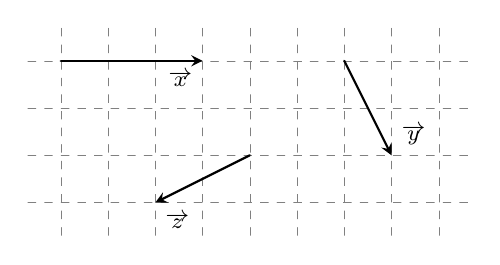
\begin{tikzpicture}[>=stealth,scale=0.6, line join=round, line cap=round]
			\draw[line width=0.05pt,gray,dashed] (-0.7,-0.7) grid (8.7,3.7);
			\draw[->,thick](0,3)--(3,3)node[below left]{\footnotesize$\overrightarrow{x}$};
			\draw[->,thick](4,1)--(2,0)node[below right]{\footnotesize$\overrightarrow{z}$};
			\draw[->,thick](6,3)--(7,1)node[above right]{\footnotesize$\overrightarrow{y}$};
		\end{tikzpicture}
	}
\loigiai{
\begin{listEX}
\item Ta có 
\begin{itemize}
	\item $|\overrightarrow{x}|=3$ cm.
	\item $|\overrightarrow{y}|=\sqrt{1^2+2^2}=\sqrt5$ cm.
	\item $|\overrightarrow{z}|=\sqrt{1^2+2^2}=\sqrt5$ cm.
\end{itemize}
\item \immini{Dựng hình vẽ tổng hợp vectơ, ta được \[|\overrightarrow{x}+\overrightarrow{y}+\overrightarrow{z}|=\sqrt{3^2+4^2}=5 \,\text{cm}.\]}{
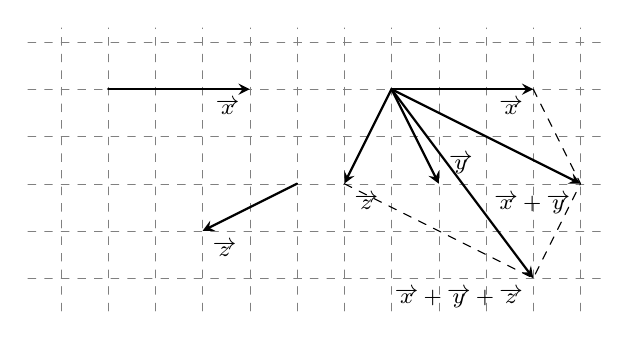
\begin{tikzpicture}[>=stealth,scale=0.6, line join=round, line cap=round]
	\draw[line width=0.05pt,gray,dashed] (-1.7,-1.7) grid (10.5,4.3);
	\draw[->,thick](0,3)--(3,3)node[below left]{\footnotesize$\overrightarrow{x}$};
	\draw[->,thick](4,1)--(2,0)node[below right]{\footnotesize$\overrightarrow{z}$};
	\draw[->,thick](6,3)--(7,1)node[above right]{\footnotesize$\overrightarrow{y}$};
\draw[->,thick](6,3)--(9,3)node[below left]{\footnotesize$\overrightarrow{x}$}; 
\draw[->,thick](6,3)--(5,1)node[below right]{\footnotesize$\overrightarrow{z}$};
\draw[dashed](9,3)--(10,1);
\draw[->,thick](6,3)--(10,1)node[below left]{\footnotesize$\overrightarrow{x}+\overrightarrow{y}$};
\draw[dashed](5,1)--(9,-1)--(10,1);
\draw[->,thick](6,3)--(9,-1)node[below left]{\footnotesize$\overrightarrow{x}+\overrightarrow{y}+\overrightarrow{z}$};
\end{tikzpicture}}
	
\end{listEX}

}

\end{vd}

\begin{vd}%[Dự án đề cương 3 Khối NH24-25-Dot1-Bùi Quang Phú]%[0H5H2-4]
	\immini{Cho hình vuông $ABCD$ tâm $O$ cạnh bằng $a$. Tính 
		\begin{listEX}[1]	
			\item $\left| \overrightarrow{AB}+\overrightarrow{BC} \right|$.
			\item $\left| \overrightarrow{AB}-\overrightarrow{AC} \right|$.
			\item $\left|\overrightarrow{AB}+\overrightarrow{OD} -\overrightarrow{BC}\right|$.
	\end{listEX}}{
		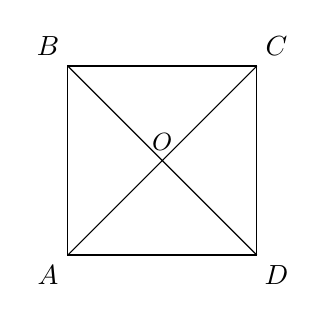
\begin{tikzpicture}[scale=1.2]
			\coordinate (M) at (0,0); \coordinate (N) at (2,0); \coordinate (P) at (2,2);
			\coordinate (Q) at (0,2); \coordinate (O) at (1,1);
			\draw (M)--(N)--(P)--(Q)--cycle; \draw (M)--(P) (N)--(Q);
			\draw (M) node[shift={(-0.25,-0.25)}] {$A$};
			\draw (Q)  node[shift={(-0.25,0.25)}] {$B$};
			\draw (N)  node[shift={(0.25,-0.25)}] {$D$};
			\draw (P)  node[shift={(0.25,0.25)}] {$C$};
			\draw (O) node[above] {\small $O$};
		\end{tikzpicture}
	}
	\loigiai{
		\begin{enumerate}[a)]
			\item Ta có $\overrightarrow{AB}+\overrightarrow{BC}=\overrightarrow{AC}$. Suy ra $\left| \overrightarrow{AB}+\overrightarrow{BC} \right|=AC=a\sqrt{2}$
			\item Ta có $\overrightarrow{AB}-\overrightarrow{AC}=\overrightarrow{CB}$. Suy ra $\left| \overrightarrow{AB}-\overrightarrow{AC} \right|=CB=a$
			\item Ta có $\overrightarrow{u} = \overrightarrow{AB}+\overrightarrow{OD} -\overrightarrow{BC}=\overrightarrow{AB}+\overrightarrow{BO}-\overrightarrow{BC}=\overrightarrow{AB}+\overrightarrow{CO}=\overrightarrow{AB}+\overrightarrow{OA}=\overrightarrow{OB}.$ \\
			Suy ra $\left|\overrightarrow{u}\right|=\left|\overrightarrow{OB}\right|=OB=\dfrac{\sqrt2}{2}AB=\dfrac{a\sqrt2}{2}.$
		\end{enumerate}
		
	}
\end{vd} 

\begin{vd}%[Dự án đề cương 3 Khối NH24-25-Dot1-Bùi Quang Phú]%[0H5V2-4]
	\immini{Cho tam giác đều $ABC$ cạnh bằng $a$, $G$ là trọng tâm tam giác $ABC$. 
		\begin{listEX}[1]
			\item Tính độ dài vectơ $\overrightarrow{AB}-\overrightarrow{AC}$, $\overrightarrow{AB}+\overrightarrow{AC}$ theo $a$.
			\item Tính độ dài vectơ $\overrightarrow{AB}+\overrightarrow{AG}$ theo $a$.
		\end{listEX}
	}{
		\begin{tikzpicture}[smooth,font=\footnotesize,scale=0.6]
			\path
			(0,0) coordinate (B)
			(4,0) coordinate (C)
			($(B)!1!60:(C)$)coordinate (A)
			($(B)!0.5!(C)$)coordinate (M);
			\draw (A)--(B)--(C)--cycle (A)--(M);
			\foreach \x/\g in {A/90,B/-90,C/-90,M/-90} \draw [fill=black] (\x) circle (.05) + (\g:.4) node{$\x$};
	\end{tikzpicture}}
	\loigiai{
		\begin{itemize}
			\item [a)] Ta có $\overrightarrow{AB}-\overrightarrow{AC}=\overrightarrow{CB}$ nên $\left| \overrightarrow{AB}-\overrightarrow{AC} \right|=CB=a$.\\
			Ta có $\overrightarrow{AB}+\overrightarrow{AC}=\overrightarrow{AD}$ với $D$ là đỉnh thứ tư của hình bình hành $ABDC$.\\
			Suy ra  $\left| \overrightarrow{AB}+\overrightarrow{AC} \right|=AD=2AM=a\sqrt{3}$.
			\item [b)] Dựng hình bình hành $AGDB$, theo qui tắc hình bình hành ta có:
			\[\overrightarrow{AB}+\overrightarrow{AG}=\overrightarrow{AD}.\]
			Gọi $M$ là trung điểm của $BC$.\\
			Dựng $DN\perp AM$ tại $N$, suy ra tứ giác $BDNM$ là hình chữ nhật $\Rightarrow MN=BD=AG=\dfrac{a\sqrt{3}}{3}$, $DN=BM=\dfrac{a}{2}$.\\
			Tam giác $AND$ vuông tại $N$, có : \\
			$AN=AM+MN=\dfrac{a\sqrt{3}}{2}+\dfrac{a\sqrt{3}}{3}=\dfrac{5a\sqrt{3}}{6}$\\
			$\Rightarrow AD=\sqrt{AN^2+ND^2}=\dfrac{a\sqrt{21}}{3}$.\\
			Vậy $\left|\overrightarrow{AB}+\overrightarrow{AG}\right|=\dfrac{a\sqrt{21}}{3}$.
	\end{itemize}}
\end{vd}

\begin{dang}{Ứng dụng của vectơ trong vật lý}
	Phép cộng vectơ tương ứng với các quy tắc tồng hợp Lực, tổng hợp vận tốc:
	\begin{itemize}
		\item [$\bullet$] Nếu hai lực cùng tác động vào chất điểm $A$ và được biểu diễn bởi các vectơ $\overrightarrow{u}_{1}, \overrightarrow{u}_{2}$ thì hợp lực tác động vào $A$ được biểu diễn bởi vectơ $\overrightarrow{u}_{1}+\overrightarrow{u}_{2}$.
		\item [$\bullet$] Nếu một con thuyền di chuyền trên sông với vận tốc riêng (vận tốc so với dòng nước) được biểu diễn bởi vectơ $\overrightarrow{v_{r}}$ và vận tốc của dòng nước (so với bờ) được biểu diễn bởi vectơ $\overline{v_{n}}$ thì vận tốc thực tế của thuyền (so với bờ) được biểu diễn bởi vectơ $\overrightarrow{v}_{r}+\overrightarrow{v}_{n}$.
	\end{itemize}
\end{dang}
\setcounter{vd}{0}
\begin{vd}%[Dự án đề cương 3 Khối NH24-25-Dot1-Bùi Quang Phú]%[0H5H2-6]
	\immini{Cho hai lực đồng quy $\overrightarrow{F_1}$ và $\overrightarrow{F_2}$ như hình vẽ. Biết độ lớn của $\overrightarrow{F_1},\text{ }\overrightarrow{F_2}$ lần lượt là 3N và 2N. Tính độ lớn hợp lực của $\overrightarrow{F_1}$ và $\overrightarrow{F_2}$.
	}{\hspace{1cm}
		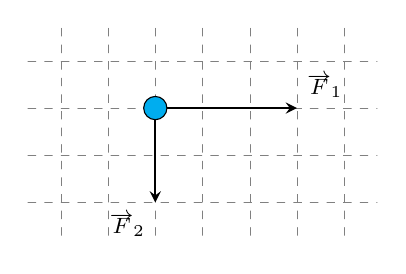
\begin{tikzpicture}[>=stealth,scale=0.6, line join=round, line cap=round]
			\draw[line width=0.05pt,gray,dashed] (-2.7,-0.7) grid (4.7,3.7);
			\draw[->,thick](0,2)--(0,0)node[below left]{\footnotesize$\overrightarrow{F}_2$};
			\draw[->,thick](0,2)--(3,2)node[above right]{\footnotesize$\overrightarrow{F}_1$};
			\draw[fill=cyan] (0,2) circle(7pt);
	\end{tikzpicture}}
\loigiai{
Dựa vào hình vẽ ta có\\
Độ lớn lực tổng hợp $\overrightarrow{F}=\overrightarrow{F_1}+\overrightarrow{F_2}$.\\
Vì hai lực $\overrightarrow{F_1}$ và $\overrightarrow{F_2}$ vuông góc với nhau nên
\[F=\sqrt{{F_1}^2+{F_2}^2}=\sqrt{3^2+2^2}=\sqrt{13}\,\text{N}.\]
}
\end{vd}

\begin{vd}%[Dự án đề cương 3 Khối NH24-25-Dot1-Bùi Quang Phú]%[0H5H2-6]
\immini{Cho hai lực $\overrightarrow{F}_{1}=\overrightarrow{M A}$,  $\overrightarrow{F}_{2}=\overrightarrow{M B}$ cùng tác động vào một vật tại điểm $M$ cường độ hai lực $\overrightarrow{F}_{1}$, $\overrightarrow{F}_{2}$ đều bằng $300$ (N) và $\widehat{AMB}=60^{\circ}$. Tìm cường độ của lực tổng hợp tác động vào vật.}
	{	\begin{tikzpicture}[smooth,font=\footnotesize,scale=0.8, >=Latex]
			\path
			(0,0) coordinate (M)
			(3,0) coordinate (A)
			($(M)!1!60:(A)$)coordinate (B);
			\fill[ball color=red](M) circle (0.16);
			\draw[->] (M)--(A);
			\draw[->] (M)--(B);
			\foreach \x/\g in {A/0,B/60,M/-90} \draw [fill=black] (\x) circle (.05) + (\g:.5) node{$\x$};
			\begin{scope}
				\clip (B)--(M)--(A);
				\draw[double] (M) circle(0.7cm);
			\end{scope}
			\node[right] at (0.6,0.5) {$60^\circ$};
		\end{tikzpicture}
	}
	\loigiai{
		\immini
		{
			Gọi $D$ là đỉnh thứ tư của hình thoi $MBDA$, ta có 
			$$\overrightarrow{MA}+\overrightarrow{MB}=\overrightarrow{MD}.$$
			Vậy cường độ lực tổng hợp tại $M$ là 
			$\left|\overrightarrow{MD}\right|=MD$.\\
			Gọi $O$ là tâm hình thoi $MBDA$ có cạnh $300$.\\
			Ta có $MD=2MO=300 \sqrt 3$ (N).
		}
		{
			\begin{tikzpicture}[smooth,font=\footnotesize,scale=0.8, >=Latex]
				\path
				(0,0) coordinate (M)
				(3,0) coordinate (A)
				($(M)!1!60:(A)$)coordinate (B)
				($(A)+(B)-(M)$)coordinate (D);
				\fill[ball color=red](M) circle (0.16);
				\draw[->] (M)--(A);
				\draw[->] (M)--(B);
				\draw[->] (M)--(D);
				\draw[dashed] (B)--(D)--(A);
				\foreach \x/\g in {A/0,B/60,M/-90,D/0} \draw [fill=black] (\x) circle (.05) + (\g:.5) node{$\x$};
				\begin{scope}
					\clip (B)--(M)--(A);
					\draw[double] (M) circle(0.7cm);
				\end{scope}
				\node[right] at (0.6,0.35) {\tiny$60^\circ$};
			\end{tikzpicture}	
		}
	}
\end{vd}

\begin{vd}%[Dự án đề cương 3 Khối NH24-25-Dot1-Bùi Quang Phú]%[0H5V2-6]
	\immini{Tính lực kéo cần thiết để kéo một khẩu pháo có trọng lượng $22\,148$ N (xấp xỉ $2\,260$ kg) lên một con dốc nghiêng $30^\circ$ so với phương nằm ngang (hình bên). Nếu lực kéo của mỗi người bằng $100$ N thì cần tối thiểu bao nhiêu người để kéo pháo (\textit{bỏ qua ma sát trượt giữa bánh xe và mặt phẳng nghiêng})?}{
		\begin{tikzpicture}[thick, font=\small, >=Latex]
			\draw (0,0)coordinate(O)
			($(O)+(0:4.5)$)coordinate(O1)
			($(O)+(30:4.55)$)coordinate(O2)
			($(O)+(30:2.8)$)coordinate(O3)
			($(O3)!0.32 cm!90:(O2)$)coordinate(A1)
			;
			\draw[cyan] (O1)--(O)--(O2)
			($(O)!0.5 cm!(O1)$) to [bend right=40]node[shift={(15:0.4)}]{\scriptsize$30^\circ$} ($(O)!0.5 cm!(O2)$)
			;
			%% -- Thân pháo
			\path 
			($(A1)+(120:0.4)$)coordinate(B1)
			($(B1)+(30:0.4)$)coordinate(B2)
			($(B1)+(210:0.5)$)coordinate(B3)
			($(B3)+(-60:0.1)$)coordinate(B4)
			($(B1)+(210:0.1)+(-60:0.02)$)coordinate(C1)
			($(C1)+(120:0.25)$)coordinate(B5)
			($(B5)+(28:1)$)coordinate(B6)
			($(C1)+(32:1)$)coordinate(B7)
			;
			%% fill pháo
			\shade [top color=darkgray, bottom color = black, middle color =lightgray, shading angle=30] (C1)..controls++(210:0.2)and++(210:0.2)..(B5)--(B6)..controls++(28:0.02)and++(32:0.01)..(B7)--(C1) ;
			%\fill bệ pháo
			\fill [darkgray] (A1) ..controls++(220:0.3) and++(30:0.5)..(B4)..controls++(210:0.1)and++(210:0.1)..(B3)--(B2)..controls++(30:0.2)and++(40:0.1)..(A1)
			;
			%%- Bánh xe
			\fill [white] (A1) circle (0.3 cm) ; 
			\foreach \a in {0,30,...,360}{
				\draw [line width=1pt, blue] (A1)--++(\a:0.3);
			}
			\draw [blue, line width=1.5pt] (A1) circle (0.3 cm);
			\fill [black] (A1) circle (0.05 cm);
			%% -- Vẽ Vecto
			\draw [dashed] ($(A1)+(-90:1.5)$)coordinate(DA)node[right]{$A$}
			(A1)++(210:0.5)coordinate(C1)
			(DA)++(120:1)coordinate(DA1)
			(intersection = of DA--DA1 and A1--C1)coordinate(DC)node[left]{$C$}
			(A1)++(120:1)coordinate(DB1)
			(DC)++(90:1)coordinate(DC1)
			(intersection = of DC--DC1 and A1--DB1)coordinate(DB)node[above left]{$B$}
			(DA)--(DC)--(DB)
			(A1)node[below right=5pt]{$O$}
			;
			\draw [->] (A1) --(DA) ;
			\draw [->] (A1) --(DB) ;
			\draw [->, dashed] (A1) --(DC) ;
			\draw [->] (A1) --++(30:1.5)node[above]{$\overrightarrow{F}$} ; %% Độ dài vecto F
	\end{tikzpicture}}
	\loigiai{
		\immini{
			Lực tổng hợp của trọng lực $\overrightarrow{P}$ và phản lực $\overrightarrow{w}$ là lực $\overrightarrow{T}=\overrightarrow{OC}$. Theo hình vẽ thì
			$$\big|\overrightarrow{T}\big|=OC=OA \cdot \sin 30^\circ=11074\, \mathrm{N}$$
			Suy ra, muốn kéo được pháo lên dốc thì lực $\overrightarrow{F}$ phải có độ lớn
			$$\big|\overrightarrow{F}\big|>\big|\overrightarrow{T}\big|=11074\, \mathrm{N}$$
			Do $\dfrac{11074}{100}=110,74$ nên nếu lực kéo mỗi người là $100$ N thì ta cần tối thiểu $111$ người.}{
			
			\begin{tikzpicture}[smooth,font=\footnotesize,scale=0.8,>= Latex]
				\path
				(0,0) coordinate (M)
				(7,0) coordinate (N)
				($(M)!1!30:(N)$) coordinate (P)
				%Dữ liệu vật trên mặt phẳng nghiên 30 độ
				($(M)!0.5!(P)$) coordinate (X)
				($(M)!0.7!(P)$) coordinate (X')
				($(X)!0.3!90:(X')$) coordinate (Y)
				($(X')!0.3!-90:(X)$) coordinate (Y')
				% Dữ liệu lực F
				($(X')!0.5!(Y)$) coordinate (O)
				($(X')!0.5!(Y')$) coordinate (I)
				($(O)!3!(I)$) coordinate (F)
				%Dữ liệu trọng lực
				($(O)!2.5!-120:(I)$) coordinate (A)
				% Dữ liệu vecto phân tích trọng lực P và phàn lực w
				($(M)!(A)!(P)$) coordinate (A')
				(intersection of A--A' and O--F) coordinate (C)
				% Dữ liệu phản lực
				($(O)+(C)-(A)$) coordinate (B)
				;
				\draw (N)--(M)--(P);
				\fill[cyan] (X)--(Y)--(Y')--(X');
				\draw[->] (O)--(F)node[above]{$\overrightarrow{F}$};
				\draw[->] (O)--(A)node[shift={(70:0.7)}]{\scriptsize$\overrightarrow{P}$};
				\draw[->] (O)--(B)node[shift={(-30:0.6)}]{\scriptsize$\overrightarrow{w}$};
				\draw[->,dashed] (O)--(C);
				\draw[dashed] (A)--(C)--(B);
				\foreach \x/\g in {O/-20,A/0,B/80,C/180} \draw [fill=black] (\x) circle (.05) + (\g:.3) node{$\x$};
				\begin{scope}
					\clip (N)--(M)--(P);
					\draw[double] (M) circle(0.6cm);
				\end{scope}
				\begin{scope}
					\clip (O)--(A)--(C);
					\draw[double] (A) circle(0.6cm);
				\end{scope}
				\node[right] at (0.6,0.25) {\scriptsize$30^\circ$};
				\node[right] at (3,1.32) {\tiny$30^\circ$};
	\end{tikzpicture}}}
\end{vd}
%%=============
\begin{dang}{Xác định điểm thỏa đẳng thức véctơ cho trước}
	Để xác định điểm $M$ thỏa đẳng thức véctơ cho trước, ta làm như sau:
	\\$\circ$\textbf{ HƯỚNG 1:}\\
	$-$ Biến đổi đẳng thức véctơ đã cho về dạng $\overrightarrow{AM}=\overrightarrow{v}$, trong đó $A$ là điểm cố định và $\overrightarrow{v}$ là véctơ cố định.\\
	$-$ Lấy $A$ làm điểm gốc, dựng véctơ bằng $\overrightarrow{v}$ thì điểm ngọn chính là điểm $M$ cần tìm.
	\\$\circ$\textbf{ HƯỚNG 2:}\\
	$-$ Biến đổi đẳng thức véctơ đã cho về dạng $\overrightarrow{AM}=\overrightarrow{AB}$, trong đó $A,B$ là hai điểm cố định.\\
	$-$ Khi đó điểm $M$ cần tìm trùng với điểm $B$.
	\\$\circ$\textbf{ HƯỚNG 3:}\\
	$-$ Biến đổi đẳng thức véctơ đã cho về một đẳng thức véctơ luôn đúng với mọi điểm $M$.\\
	$-$ Khi đó điểm $M$ cần tìm là điểm tùy ý.
	\\$\circ$\textbf{ HƯỚNG 4:}\\
	$-$ Biến đổi đẳng thức véctơ đã cho về một đẳng thức véctơ luôn sai với mọi điểm $M$.\\
	$-$ Khi đó không có điểm $M$ nào thỏa điều kiện.
	\\$\circ$\textbf{ HƯỚNG 5:}\\
	$-$ Biến đổi đẳng thức véctơ đã cho về dạng $\left\vert \overrightarrow{IM}\right\vert=\left\vert \overrightarrow{AB}\right\vert$, trong đó $I,A,B$ là các điểm cố định.\\
	$-$ Khi đó điểm $M$ cần tìm thuộc đường tròn tâm $I$, bán kính $AB$.
	\\$\circ$\textbf{ HƯỚNG 6:}\\
	$-$ Biến đổi đẳng thức véctơ đã cho về dạng $\left\vert \overrightarrow{MA}\right\vert=\left\vert \overrightarrow{MB}\right\vert$, trong đó $A,B$ là các điểm cố định phân biệt.\\
	$-$ Khi đó điểm $M$ cần tìm thuộc đường trung trực của đoạn $AB$.
\end{dang}
\begin{vd}%[Dự án đề cương 3 Khối NH24-25-Dot1-Bùi Quang Phú]%[0H5H2-3]
	Cho hình bình hành $ABCD$ có tâm $O$. Tìm ba điểm $M$, $N$, $P$ thỏa mãn:
	\begin{listEX}[3]
		\item $\overrightarrow{MA}+\overrightarrow{MD}+\overrightarrow{MB}=\overrightarrow{0}$;
		\item $\overrightarrow{ND}+\overrightarrow{NB}+\overrightarrow{NC}=\overrightarrow{0}$;
		\item $\overrightarrow{PM}+\overrightarrow{PN}=\overrightarrow{0}$.
	\end{listEX}
	\loigiai{
		\immini{
			\begin{enumerate}
				\item Ta chọn $M$ là trọng tâm tam giác $ADB$. Khi đó $\overrightarrow{MA}+\overrightarrow{MD}+\overrightarrow{MB}=\overrightarrow{0}$.
				\item Ta chọn $N$ là trọng tâm tam giác $DBC$. Khi đó $\overrightarrow{ND}+\overrightarrow{NB}+\overrightarrow{NC}=\overrightarrow{0}$.
				\item Ta chọn $P\equiv O$. Ta có $O$ là trung điểm $MN$, khi đó $$\overrightarrow{PM}+\overrightarrow{PN}=\overrightarrow{OM}+\overrightarrow{ON}=\overrightarrow{0}.$$
			\end{enumerate}
		}{
			\begin{tikzpicture}[scale=1, font=\footnotesize, line join=round, line cap=round, >=stealth]
				\path
				(0,0) coordinate (A)
				(2.5,0) coordinate (B)
				(1,1.7) coordinate (D)
				($(A)!1/2!(C)$) coordinate (O)
				($(A)!1/3!(C)$) coordinate (M)
				($(A)!2/3!(C)$) coordinate (N)
				($(B)+(D)-(A)$) coordinate (C)
				;
				\draw (A)--(B)--(C)--(D)--(A)--(C) (B)--(D);
				\foreach \x/\g in
				{A/-90,B/-90,C/90,D/90,O/90,M/-90,N/90}
				\fill[black](\x) circle (1.2pt)
				($(\x)+(\g:3mm)$) node{$\x$};
			\end{tikzpicture}
		}
	}
\end{vd}
\begin{vd}%[Dự án đề cương 3 Khối NH24-25-Dot1-Bùi Quang Phú]%[0H5H2-3]
	Cho tam giác $ABC$. Tìm điểm $M$ thỏa mãn điều kiện $\overrightarrow{BA}+\overrightarrow{BC}+\overrightarrow{MB}=\overrightarrow{0}$.
	\loigiai{
		\immini{$\overrightarrow{BA}+\overrightarrow{BC}+\overrightarrow{MB}=\overrightarrow{0}\Leftrightarrow \overrightarrow{BA}+\overrightarrow{MC}=\overrightarrow{0} \Leftrightarrow \overrightarrow{CM}=\overrightarrow{BA}$\\
			$\Rightarrow$ Điểm $M$ là điểm thứ tư của hình bình hành $ABCM$.}
		{\begin{tikzpicture}[line cap=round, line join=round, scale=0.8]
				% Định nghĩa các điểm A, B, C
				\coordinate (A) at (1,2);
				\coordinate (B) at (0,0);
				\coordinate (C) at (4,0);
				
				% Tính điểm M thỏa mãn BA + BC + MB = 0
				% Ta có: BA = A - B, BC = C - B, MB = B - M
				% => (A-B) + (C-B) + (B-M) = 0
				% => A - B + C - B + B - M = 0
				% => A + C - B - M = 0
				% => M = A + C - B
				\coordinate (M) at ($(A) + (C) - (B)$);
				
				% Vẽ các đoạn thẳng
				\draw (A) -- (B) -- (C) -- cycle;
				\draw (A) -- (M) -- (C);
				
				% Vẽ các điểm
				\fill[black] (A) circle (2pt);
				\fill[black] (B) circle (2pt);
				\fill[black] (C) circle (2pt);
				\fill[black] (M) circle (2pt);
				
				% Nhãn các điểm
				\node[above] at (A) {$A$};
				\node[above] at (M) {$M$};
				\node[below] at (B) {$B$};
				\node[below] at (C) {$C$};
		\end{tikzpicture}}
	}
\end{vd}
%
\begin{vd}%[Dự án đề cương 3 Khối NH24-25-Dot1-Bùi Quang Phú]%[0H5H2-3]
	Cho tam giác $ABC$. Tìm điểm $M$ thỏa mãn điều kiện $\overrightarrow{MA}-\overrightarrow{MB}+\overrightarrow{MC}=\overrightarrow{BC}$.
	\loigiai{
		\immini{$\overrightarrow{MA}-\overrightarrow{MB}+\overrightarrow{MC}=\overrightarrow{BC}\Leftrightarrow \overrightarrow{BA}-\overrightarrow{BC}=\overrightarrow{CM}\Leftrightarrow \overrightarrow{CA}=\overrightarrow{CM}$\\
			$\Rightarrow$ Điểm $M$ trùng với điểm $A$.}
		{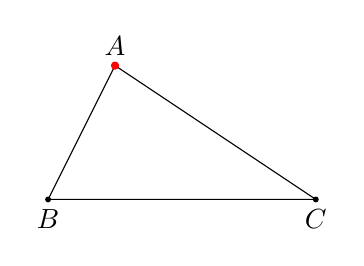
\begin{tikzpicture}[line cap=round, line join=round, scale=0.85]
				% Định nghĩa các điểm A, B, C
				\coordinate (B) at (0,0);
				\coordinate (C) at (4,0);
				\coordinate (A) at (1,2);
				
				% Vẽ tam giác ABC
				\draw (A) -- (B) -- (C) -- cycle;
				
				% Đánh dấu các điểm
				\filldraw (A) circle (1pt) node[above] {$A$};
				\filldraw (B) circle (1pt) node[below] {$B$};
				\filldraw (C) circle (1pt) node[below] {$C$};
				\filldraw[red] (A) circle (1.5pt);
		\end{tikzpicture}}
	}
\end{vd}
%
\begin{vd}%[Dự án đề cương 3 Khối NH24-25-Dot1-Bùi Quang Phú]%[0H5H2-3]
	Cho tam giác $ABC$. Tìm điểm $M$ thỏa mãn điều kiện $\overrightarrow{MA}-\overrightarrow{MB}=\overrightarrow{AB}$.
	\loigiai{
		\immini{$\overrightarrow{MA}-\overrightarrow{MB}=\overrightarrow{AB}\Leftrightarrow \overrightarrow{BA}=\overrightarrow{AB}$\\
			$\Rightarrow$ không có $M$ nào thỏa điều kiện bài toán.}
		{\begin{tikzpicture}[line cap=round, line join=round, scale=0.85]
				% Định nghĩa các điểm A, B, C
				\coordinate (B) at (0,0);
				\coordinate (C) at (4,0);
				\coordinate (A) at (1,2);
				
				% Vẽ tam giác ABC
				\draw (A) -- (B) -- (C) -- cycle;
				
				% Đánh dấu các điểm
				\filldraw (A) circle (1pt) node[above] {$A$};
				\filldraw (B) circle (1pt) node[below left] {$B$};
				\filldraw (C) circle (1pt) node[below right] {$C$};
		\end{tikzpicture}}
	}
\end{vd}
%
\begin{vd}%[Dự án đề cương 3 Khối NH24-25-Dot1-Bùi Quang Phú]%[0H5V2-3]
	Cho tam giác $ABC$. Tìm điểm $M$ thỏa mãn điều kiện $\left|\overrightarrow{MA}\right|=\left|\overrightarrow{MB}-\overrightarrow{MC}\right|$.
	\loigiai{
		\immini{$\left|\overrightarrow{MA}\right|=\left|\overrightarrow{MB}-\overrightarrow{MC}\right| \Leftrightarrow \left| \overrightarrow{MA}\right| =\left| \overrightarrow{CB}\right| \Leftrightarrow MA =CB$\\
		Suy ra điểm $M$ thuộc đường tròn tâm $A$, bán kính $CB$.}
		{\begin{tikzpicture}[line cap=round, line join=round, scale=1.2]
				% Define points A, B, C
				\coordinate (B) at (0,0);
				\coordinate (C) at (2,0);
				\coordinate (A) at (1,1);
				
				% Find point M satisfying |MA| = |MB - MC|
				% Since MB - MC = CB, we need |MA| = |CB|
				% So M lies on circle centered at A with radius CB
				\draw let \p1=($(C)-(B)$), \n1={veclen(\x1,\y1)} in 
				(A) circle (\n1);
				
				% Calculate one solution point M (translation of A by vector BC)
				\coordinate (M) at ($(A)+(C)-(B)$);
				
				% Draw triangle ABC
				\draw (A) -- (B) -- (C) -- cycle;
				
				% Draw points and labels
				\filldraw (A) circle (1.5pt) node[above] {$A$};
				\filldraw (B) circle (1.5pt) node[below left] {$B$};
				\filldraw (C) circle (1.5pt) node[below right] {$C$};
				\filldraw[red] (M) circle (1.5pt) node[right] {$M$};
				
				% Draw vectors
				\draw[->, thick, blue] (A) -- (M);
				\draw[->, thick, green!70!black] (B) -- (C);
				\draw[dashed] (A) -- (M) (C) -- (M);
		
				\end{tikzpicture}}
	}
\end{vd}






%-----------------------------------------------------------------------------
\subsection{Bài tập rèn luyện}
\ind{PHẦN I.} \inden{Câu trắc nghiệm nhiều phương án lựa chọn. Mỗi câu hỏi học sinh chỉ chọn một phương án.}\\
\setcounter{ex}{0}
\Opensolutionfile{ans}[ans/0H5-Bai2-TN]

%%%============EX_1==============%%%
\begin{ex}%[Dự án đề cương 3 Khối NH24-25-Dot1-Bùi Quang Phú]%[0H5N2-2]
	Cho tam giác $ABC$. Khẳng định nào sau đây là khẳng định đúng?
	\choice
	{$\overrightarrow{AB}+\overrightarrow{AC}=\overrightarrow{BC}$}
	{\True $\overrightarrow{BC}+\overrightarrow{AB}=\overrightarrow{AC}$}
	{$\overrightarrow{AB}-\overrightarrow{AC}=\overrightarrow{BC}$}
	{$\overrightarrow{AB}+\overrightarrow{AC}=\overrightarrow{CB}$}
\loigiai{Ta có $\overrightarrow{BC}+\overrightarrow{AB}=\overrightarrow{AB}+\overrightarrow{BC}=\overrightarrow{AC}$.}
\end{ex}
%%%============EX_2==============%%%
\begin{ex}%[Dự án đề cương 3 Khối NH24-25-Dot1-Bùi Quang Phú]%[0H5N2-2]
	Cho hình bình hành $ABCD$. Mệnh đề nào sau đây là mệnh đề đúng?
	\choice
	{$\overrightarrow{AB}+\overrightarrow{AD}=\overrightarrow{BD}$}
	{$\overrightarrow{AB}+\overrightarrow{AD}=\overrightarrow{DB}$}
	{\True $\overrightarrow{BA}+\overrightarrow{BC}=\overrightarrow{BD}$}
	{$\overrightarrow{BA}+\overrightarrow{BC}=\overrightarrow{DB}$}
\loigiai{Theo quy tắc hình bình hành, ta có $\overrightarrow{BA}+\overrightarrow{BC}=\overrightarrow{BD}$.
}
\end{ex}
%%%============EX_3==============%%%
\begin{ex}%[Dự án đề cương 3 Khối NH24-25-Dot1-Bùi Quang Phú]%[0H5N2-1]
(\textit{Trích đề thi HKI - Trường THPT Minh Hà - Hà Nội - Năm học: 2024-2025})\\
Cho ba điểm $A$, $B$, $C$. vectơ tổng  $\overrightarrow{AB}+\overrightarrow{CA}+\overrightarrow{BC}$ bằng
	\choice
	{$\overrightarrow{BA}$}
	{$\overrightarrow{AC}$}
	{$\overrightarrow{CA}$}
	{\True $\overrightarrow{0}$}
\loigiai{
 Ta có $\overrightarrow{AB}+\overrightarrow{CA}+\overrightarrow{BC}=\overrightarrow{AB}+\overrightarrow{BC}+\overrightarrow{CA}=\overrightarrow{AC}+\overrightarrow{CA}=\overrightarrow{AA}=\overrightarrow{0}$.
}
\end{ex}
%%%============EX_4==============%%%
\begin{ex}%[Dự án đề cương 3 Khối NH24-25-Dot1-Bùi Quang Phú]%[0H5N2-1]
(\textit{Trích đề thi HKI - THPT Thanh Bình 1 - Đồng Tháp - Năm học: 2024-2025})\\
Tổng các vectơ $\overrightarrow{MN}+\overrightarrow{NP}+\overrightarrow{PQ}$ bằng
	\choice
	{$\overrightarrow{MP}$}
	{$\overrightarrow{MN}$}
	{\True $\overrightarrow{MQ}$}
	{$\overrightarrow{QM}$}
\loigiai{
Ta có $\overrightarrow{MN}+\overrightarrow{NP}+\overrightarrow{PQ}=\overrightarrow{MP}+\overrightarrow{PQ}=\overrightarrow{MQ}$. 
}
\end{ex}
%%%============EX_5==============%%%
\begin{ex}%[Dự án đề cương 3 Khối NH24-25-Dot1-Bùi Quang Phú]%[0H5N2-1]
	Cho tam giác $ABC$ có $M$, $N$, $P$ lần lượt là trung điểm của các cạnh $AB$, $AC$, $BC$. Hỏi $\overrightarrow{MP}+\overrightarrow{NP}$ bằng vectơ nào sau đây?
	\choice
	{$\overrightarrow{AM}$}
	{$\overrightarrow{MN}$}
	{$\overrightarrow{PB}$}
	{\True $\overrightarrow{AP}$}
\loigiai{
\immini{Vì $N P$ là đường trung bình của $\triangle A B C$ nên $N P=\dfrac{1}{2} A B=A M$ và $N P \parallel A M$.\\
Nên $\overrightarrow{N P}=\overrightarrow{A M}$.\\
Ta có $\overrightarrow{MP}+\overrightarrow{NP}=\overrightarrow{NP}+\overrightarrow{MP}=\overrightarrow{AM}+\overrightarrow{MP}=\overrightarrow{AP}$.}{\begin{tikzpicture}[scale=0.5,line width=0.7pt, font=\footnotesize, line join=round, line cap=round, >=stealth]
	%% Khai bao diem		
	\path
	(0,0) coordinate (B)
	(5,0) coordinate (C)
	(1.75,3.25) coordinate (A)
	($(A)!1/2!(B)$) coordinate (M)
	($(A)!1/2!(C)$) coordinate (N)
	($(C)!1/2!(B)$) coordinate (P)
	;
	
	\draw (A)--(B)--(C)--(A) (M)--(N)--(P)--(M);
	%% vẽ điểm
	\foreach \x/\g in {A/90,B/-90,C/-90,M/160,N/60,P/-90}
	\draw[fill=black] (\x) circle (.036)+(\g:.33)
	node{$\x$};	
	
	\end{tikzpicture}}
}
\end{ex}
%%%============EX_6==============%%%
\begin{ex}%[Dự án đề cương 3 Khối NH24-25-Dot1-Bùi Quang Phú]%[0H5H2-1]
	Cho hình bình hành $ABCD$. Tìm $\overrightarrow{v}=\overrightarrow{DC}+\overrightarrow{AD}$.
	\choice
	{$\overrightarrow{v}=\overrightarrow{CA}$}
	{\True $\overrightarrow{v}=\overrightarrow{AC}$}
	{$\overrightarrow{v}=\overrightarrow{DB}$}
	{$\overrightarrow{v}=\overrightarrow{BD}$}
\loigiai{
\immini{Ta có $\overrightarrow{DC}=\overrightarrow{AB}$.\\
	Nên theo quy tắc hình bình hành $\overrightarrow{v}=\overrightarrow{DC}+\overrightarrow{AD}=\overrightarrow{AB}+\overrightarrow{AD}=\overrightarrow{AC}$.}{	\begin{tikzpicture}[scale=0.5,line width=0.7pt, font=\footnotesize, line join=round, line cap=round, >=stealth]
	%% Khai bao diem		
	\path
	(0,0) coordinate (D)
	(5,0) coordinate (C)
	(1.75,2.25) coordinate (A)
	($(C)+(A)$) coordinate (B)
	;
	
	\draw (A)--(B)--(C)--(D)--(A) ;
	%% vẽ điểm
	\foreach \x/\g in {A/90,B/90,C/-90,D/-90}
	\draw[fill=black] (\x) circle (.036)+(\g:.35)
	node{$\x$};	
	
	\end{tikzpicture}}
}
\end{ex}
%%%============EX_7==============%%%
\begin{ex}%[Dự án đề cương 3 Khối NH24-25-Dot1-Bùi Quang Phú]%[0H5H2-1]
(\textit{Trích đề thi GKI - THPT Lê Thánh Tông - HCM - Năm học: 2024-2025})\\
Cho hình bình hành $ABCD$ và hai điểm bất kì $M$, $N$ lần lượt thuộc các đường thẳng $AB$, $AD$. Khi đó $\overrightarrow{AM}+\overrightarrow{MB}+\overrightarrow{AN}-\overrightarrow{DN}$ bằng với
	\choice
	{$\overrightarrow{MN}$}
	{\True $\overrightarrow{AC}$}
	{$\overrightarrow{BD}$}
	{$\overrightarrow{NM}$}
	\loigiai{
		\begin{center}
			\begin{tikzpicture}[line join=round,line cap=round,>=stealth,scale=0.9,font=\footnotesize]
				\tikzset{every node/.style={outer sep=-0.5mm}}
				\foreach \x/\y/\n in {0/0/D,5/0/C,2/2/A, 7/2/B} \coordinate (\n) at (\x,\y);
				\coordinate (M) at ($(A)!0.3!(B)$); \coordinate (N) at ($(A)!0.7!(D)$);
				\draw (A)--(B)--(C)--(D)--cycle;
				\foreach \t/\g in {B/90,C/-90,A/90,D/-90,M/90,N/100}{
					\fill (\t) circle (1.5pt) node[shift={(\g:10pt)}]{$\t$};}
			\end{tikzpicture}
		\end{center}
		Ta có $\overrightarrow{AM}+\overrightarrow{MB}+\overrightarrow{AN}-\overrightarrow{DN} 
		= \overrightarrow{AB}+\overrightarrow{AN}+\overrightarrow{ND}
		=\overrightarrow{AB}+\overrightarrow{AD}
		=\overrightarrow{AC}$.
	}
\end{ex}
%%%============EX_8==============%%%
\begin{ex}%[Dự án đề cương 3 Khối NH24-25-Dot1-Bùi Quang Phú]%[0H5H2-1]
	Cho hình bình hành $ABCD$ có $O$ là giao điểm của hai đường chéo $AC$ và $BD$. Khi đó, vectơ $\overrightarrow{BO}-\overrightarrow{DO}+\overrightarrow{DC}$ bằng
	\choice
	{\True $\overrightarrow{BC}$}
	{$\overrightarrow{CB}$}
	{$\overrightarrow{BD}$}
	{$\overrightarrow{AB}$}
\loigiai{
\immini{Ta có $\overrightarrow{B O}-\overrightarrow{D O}+\overrightarrow{D C}=\overrightarrow{B O}+\overrightarrow{O D}+\overrightarrow{D C}=\overrightarrow{B D}+\overrightarrow{D C}=\overrightarrow{B C}$.}{\begin{tikzpicture}[scale=0.5,line width=0.7pt, font=\footnotesize, line join=round, line cap=round, >=stealth]
		%% Khai bao diem		
		\path
		(0,0) coordinate (D)
		(5,0) coordinate (C)
		(1.75,2.25) coordinate (A)
		($(C)+(A)$) coordinate (B)
		(intersection of A--C and B--D) coordinate (O)
		;
		
		\draw (A)--(B)--(C)--(D)--(A)--(C) (B)--(D) ;
		%% vẽ điểm
		\foreach \x/\g in {A/90,B/90,C/-90,D/-90,O/90}
		\draw[fill=black] (\x) circle (.036)+(\g:.35)
		node{$\x$};	
		
\end{tikzpicture}}
}
\end{ex}
%%%============EX_9==============%%%
\begin{ex}%[Dự án đề cương 3 Khối NH24-25-Dot1-Bùi Quang Phú]%[0H5H2-2]
	Cho hình bình hành $ABCD$ tâm $O$. Đẳng thức nào sau đây đúng?
	\choice[2]
	{$\overrightarrow{AB}+\overrightarrow{BO}+\overrightarrow{DC}+\overrightarrow{DO}=\overrightarrow{0}$}
	{$\overrightarrow{AO}+\overrightarrow{BO}+\overrightarrow{CO}+\overrightarrow{OD}=\overrightarrow{0}$}
	{$\overrightarrow{AO}+\overrightarrow{OB}+\overrightarrow{CO}+\overrightarrow{DO}=\overrightarrow{0}$}
	{\True $\overrightarrow{OA}+\overrightarrow{AB}+\overrightarrow{OC}+\overrightarrow{CD}=\overrightarrow{0}$}
\loigiai{
\immini{Vì $A B C D$ là hình bình hành tâm $O$ nên $\overrightarrow{O A}+\overrightarrow{OC}=\overrightarrow{0}$ và $\overrightarrow{AB}+\overrightarrow{CD}=\overrightarrow{0}$.\\
Do đó $\overrightarrow{O A}+\overrightarrow{AB}+\overrightarrow{OC}+\overrightarrow{CD}=\left(\overrightarrow{OA}+\overrightarrow{OC}\right)+\left(\overrightarrow{AB}+\overrightarrow{CD}\right)=\overrightarrow{0}$.}{\begin{tikzpicture}[scale=0.5,line width=0.7pt, font=\footnotesize, line join=round, line cap=round, >=stealth]
	%% Khai bao diem		
	\path
	(0,0) coordinate (D)
	(5,0) coordinate (C)
	(1.75,2.25) coordinate (A)
	($(C)+(A)$) coordinate (B)
	(intersection of A--C and B--D) coordinate (O)
	;
	
	\draw (A)--(B)--(C)--(D)--(A)--(C) (B)--(D) ;
	%% vẽ điểm
	\foreach \x/\g in {A/90,B/90,C/-90,D/-90,O/90}
	\draw[fill=black] (\x) circle (.036)+(\g:.35)
	node{$\x$};	
	
	\end{tikzpicture}}
}
\end{ex}
%%%============EX_10==============%%%
\begin{ex}%[Dự án đề cương 3 Khối NH24-25-Dot1-Bùi Quang Phú]%[0H5H2-1]
	Cho hình bình hành $ABCD$. Gọi $M$, $N$ lần lượt là trung điểm của đoạn thẳng $BC$ và $AD$. Vectơ $\overrightarrow{NC}+\overrightarrow{BM}$ bằng
	\choice
	{$\overrightarrow{MN}$}
	{$\overrightarrow{NM}$}
	{\True $\overrightarrow{AC}$}
	{$\overrightarrow{CA}$}
\loigiai{
\immini{Vì $AD=BC$ và $AD \parallel BC$ nên $AN=BM$ và $AN \parallel BM$.\\
	Suy ra $\overrightarrow{BM}=\overrightarrow{AN}$.\\
	Ta có $\overrightarrow{NC}+\overrightarrow{BM}=\overrightarrow{BM}+\overrightarrow{NC}=\overrightarrow{AN}+\overrightarrow{NC}=\overrightarrow{AC}$.}{\begin{tikzpicture}[scale=0.5,line width=0.7pt, font=\footnotesize, line join=round, line cap=round, >=stealth]
		%% Khai bao diem		
		\path
		(0,0) coordinate (D)
		(5,0) coordinate (C)
		(1.75,2.25) coordinate (A)
		($(C)+(A)$) coordinate (B)
		($(A)!1/2!(D)$) coordinate (N)
		($(B)!1/2!(C)$) coordinate (M)
		;
		
		\draw (A)--(B)--(C)--(D)--(A) (N)--(C) ;
		%% vẽ điểm
		\foreach \x/\g in {A/90,B/90,C/-90,D/-90,N/150,M/-20}
		\draw[fill=black] (\x) circle (.037)+(\g:.35)
		node{$\x$};	
		
		\end{tikzpicture}}
}
\end{ex}
%%%============EX_11==============%%%
\begin{ex}%[Dự án đề cương 3 Khối NH24-25-Dot1-Bùi Quang Phú]%[0H5H2-3]
	Cho đoạn thẳng $AB$ và điểm $M$ thỏa $\overrightarrow{MB}+\overrightarrow{MA}=\overrightarrow{0}$. Mệnh đề nào sau đây là mệnh đề đúng?
	\choice
	{\True $M$ là trung điểm $AB$}
	{$M$ trùng $A$}
	{$M$ trùng $B$}
	{$A$ là trung điểm $MB$}
\loigiai{$\overrightarrow{MA}+\overrightarrow{MB}=\overrightarrow{0}$ khi và chỉ khi $M$ là trung điểm của $AB$.}
\end{ex}
%%%============EX_12==============%%%
\begin{ex}%[Dự án đề cương 3 Khối NH24-25-Dot1-Bùi Quang Phú]%[0H5H2-3]
	Cho $\overrightarrow{AB}$ khác $\overrightarrow{0}$ và cho điểm $C$. Có bao nhiêu điểm $D$ thỏa $\overrightarrow{AB}=\overrightarrow{CD}$?
	\choice
	{Vô số}
	{\True $1$}
	{$2$}
	{$0$}
\loigiai{
\immini{Qua điểm $C$, dựng đường thẳng $d$ song song với giá của véc tơ $\overrightarrow{A B}$.\\
Trên $d$, xác định điểm $D$ sao cho $\overrightarrow{A B}=\overrightarrow{C D}$ (thỏa cùng hướng và cùng độ dài).\\
Như vậy có duy nhất một điểm $D$ thỏa mãn.}{\begin{tikzpicture}[scale=0.5,line width=0.7pt, font=\footnotesize, line join=round, line cap=round, >=stealth]
	%% Khai bao diem		
	\path
	(0,0) coordinate (C)
	(5,0) coordinate (D)
	(1.75,2.25) coordinate (A)
	($(D)+(A)$) coordinate (B)
	;
	
	\draw (A)--(B) ($(C)+(-1,0)$)--($(D)+(1.5,0)$) node[above]{$d$} ;
	%% vẽ điểm
	\foreach \x/\g in {A/90,B/90,C/-90,D/-90}
	\draw[fill=black] (\x) circle (.037)+(\g:.35)
	node{$\x$};	
	
	\end{tikzpicture}}
}
\end{ex}
%%%============EX_13==============%%%
\begin{ex}%[Dự án đề cương 3 Khối NH24-25-Dot1-Bùi Quang Phú]%[0H5H2-3]
	Cho hình chữ nhật $ABCD$ ta có $\overrightarrow{DC}+\overrightarrow{BD}+\overrightarrow{AB}=\overrightarrow{BM}$. Khi đó điểm $M$
	\choice
	{Trùng với điểm $D$}
	{Đối xứng với $A$ qua $C$}
	{\True Đối xứng với $D$ qua $C$}
	{Trùng với điểm $C$}
\loigiai{
\immini{Ta có $\overrightarrow{DC}+\overrightarrow{BD}+\overrightarrow{AB}=\overrightarrow{BM} \Leftrightarrow \overrightarrow{AB}+\overrightarrow{BD}+\overrightarrow{DC}=\overrightarrow{BM} \Leftrightarrow \overrightarrow{AD}+\overrightarrow{DC}=\overrightarrow{BM} \Leftrightarrow \overrightarrow{AC}=\overrightarrow{BM}$.\\[0.2cm]
Suy ra $A B M C$ là hình bình hành.\\[0.2cm]
Suy ra $M$ đối xứng với $D$ qua $C$.}{\begin{tikzpicture}[scale=0.5,line width=0.7pt, font=\footnotesize, line join=round, line cap=round, >=stealth]
	%% Khai bao diem		
	\path
	(0,0) coordinate (D)
	(5,0) coordinate (C)
	(0,3) coordinate (A)
	($(C)+(A)$) coordinate (B)
	($(D)!2!(C)$) coordinate (M)
	;
	
	\draw (A)--(B)--(C)--(D)--(A)--(C) (C)--(M)--(B) ;
	%% vẽ điểm
	\foreach \x/\g in {A/90,B/90,C/-90,D/-90,M/-90}
	\draw[fill=black] (\x) circle (.037)+(\g:.35)
	node{$\x$};	
	
	\end{tikzpicture}}
}
\end{ex}
%%%============EX_14==============%%%
\begin{ex}%[Dự án đề cương 3 Khối NH24-25-Dot1-Bùi Quang Phú]%[0H5N2-3]
	Cho tam giác $ABC$ và điểm $M$ thỏa mãn $\overrightarrow{MB}+\overrightarrow{MC}=\overrightarrow{AB}$. Tìm vị trí điểm $M$.
	\choice
	{$M$ là trung điểm của $AB$}
	{$M$ là trung điểm của $BC$}
	{$M$ là trung điểm của $AC$}
	{$M$ là điểm thứ tư của hình bình hành $ABCM$}
\loigiai{ 
Ta có $\overrightarrow{MB}+\overrightarrow{MC}=\overrightarrow{AB} \Leftrightarrow \overrightarrow{MB}+\overrightarrow{MC}=\overrightarrow{MB}-\overrightarrow{MA} \Leftrightarrow \overrightarrow{MC}+\overrightarrow{MA}=\overrightarrow{0}$.\\
Vậy $M$ là trung điểm của $AC$.
}
\end{ex}
%%%============EX_15==============%%%
\begin{ex}%[Dự án đề cương 3 Khối NH24-25-Dot1-Bùi Quang Phú]%[0H5H2-4]
	Cho tam giác $ABC$ vuông tại $A$ có $AB=2$, $AC=3$ và $M$ là trung điểm của $BC$. Khi đó $2\left|\overrightarrow{MC}-\overrightarrow{AC}\right|$ bằng
	\choice
	{$5$}
	{$40$}
	{\True $\sqrt{13}$}
	{$2\sqrt{10}$}
\loigiai{
Ta có $2\left|\overrightarrow{MC}-\overrightarrow{AC}\right|=2\left|\overrightarrow{MC}+\overrightarrow{CA}\right|=2\left|\overrightarrow{MA}\right|=2AM$.\\
Xét $\triangle A B C$ vuông tại $A$ có $B C=\sqrt{A B^{2}+A C^{2}}=\sqrt{2^{2}+3^{2}}=\sqrt{13}$.\\
Theo định lí trung tuyến ứng cạnh huyền ta có $AM=\dfrac{BC}{2} \Rightarrow 2AM=BC=\sqrt{13}$.\\
Vậy $2\left|\overrightarrow{MC}-\overrightarrow{AC}\right|=BC=\sqrt{13}$.
}
\end{ex}
%%%============EX_16==============%%%
\begin{ex}%[Dự án đề cương 3 Khối NH24-25-Dot1-Bùi Quang Phú]%[0H5H2-4]
	Cho tam giác $ABC$ vuông cân tại $A$ có $AB=a$. Tính $\left|\overrightarrow{AB}+\overrightarrow{AC}\right|$.
	\choice
	{\True $\left|\overrightarrow{AB}+\overrightarrow{AC}\right|=a \sqrt{2}$}
	{$\left|\overrightarrow{AB}+\overrightarrow{AC}\right|=\dfrac{a\sqrt{2}}{2}$}
	{$\left|\overrightarrow{AB}+\overrightarrow{AC}\right|=2a$}
	{$\left|\overrightarrow{AB}+\overrightarrow{AC}\right|=a$}
\loigiai{
\immini{Dựng điểm $D$ là điểm thứ tư của hình bình hành $ABDC$.\\
Theo quy tắc hình bình hành $\overrightarrow{AB}+\overrightarrow{AC}=\overrightarrow{AD}$.\\
Suy ra $\left|\overrightarrow{A B}+\overrightarrow{A C}\right|=\left|\overrightarrow{A D}\right|=A D$.\\
Dễ thấy $BACM$ là hình vuông cạnh $a$. Khi đó đường chéo $A D=a \sqrt{2}$.\\
Vậy $\left|\overrightarrow{AB}+\overrightarrow{AC}\right|=a\sqrt{2}$.}{\begin{tikzpicture}[scale=0.7,line width=0.7pt, font=\footnotesize, line join=round, line cap=round, >=stealth]
	%% Khai bao diem		
	\path
	(0,0) coordinate (A)
	(3,0) coordinate (C)
	(0,3) coordinate (B)
	($(C)+(B)$) coordinate (D)
	;
	
	\draw (A)--(C)--(D)--(B)--(A)--(D) ;
	%% vẽ điểm
	\foreach \x/\g in {A/-90,B/90,C/-90,D/90}
	\draw[fill=black] (\x) circle (.037)+(\g:.35)
	node{$\x$};	
	
	\end{tikzpicture}}
}
\end{ex}
%%%============EX_17==============%%%
\begin{ex}%[Dự án đề cương 3 Khối NH24-25-Dot1-Bùi Quang Phú]%[0H5H2-4]
(\textit{Trích đề thi HKI - THPT Nguyễn Quốc Trinh - Hà Nội - Năm học: 2024-2025})\\
Cho hình thoi $ABCD$ có cạnh bằng $a$ và $\widehat{BAD}=60^{\circ}$. Khi đó $\left|\overrightarrow{AD}-\overrightarrow{AB}\right|$ bằng
	\choice
	{$a\sqrt{2}$}
	{$a$}
	{\True $2a$}
	{$\dfrac{a\sqrt{3}}{2}$}
\loigiai{
\immini{Ta có $\left|\overrightarrow{AD}-\overrightarrow{AB}\right|=\left|\overrightarrow{BD}\right|=BD$ (quy tắc hình bình hành).\\
	Vì $\triangle ABD$ có $\heva{
		& \widehat{BAC}=60^{\circ}   \\
		&  AB=AC \text { (hình thoi) } \\
	}$ nên $\triangle BAD$ đều.\\
Suy ra $BD=AB=2a$.
Vậy $\left|\overrightarrow{AD}-\overrightarrow{AB}\right|=2a$.}{\begin{tikzpicture}[scale=0.7,line width=0.7pt, font=\footnotesize, line join=round, line cap=round, >=stealth]
	%% Khai bao diem		
	\path
	(0,0) coordinate (A)
	(30:2.75) coordinate (B)
	(-30:2.75) coordinate (D)
	($(B)+(D)-(A)$) coordinate (C)
	;
	
	\draw (A)--(B)--(C)--(D)--(A) (B)--(D) ;
	%% vẽ điểm
	\foreach \x/\g in {A/180,B/90,C/0,D/-90}
	\draw[fill=black] (\x) circle (.037)+(\g:.35)
	node{$\x$};	
	
	\end{tikzpicture}}
}
\end{ex}
%%%============EX_18==============%%%
\begin{ex}%[Dự án đề cương 3 Khối NH24-25-Dot1-Bùi Quang Phú]%[0H5H2-4]
	Cho tam giác $ABC$ đều cạnh $a$ có $G$ là trọng tâm. Tính $\left|\overrightarrow{GA}+\overrightarrow{GB}\right|$ theo $a$.
	\choice
	{$\dfrac{a}{3}$}
	{$a$}
	{\True $\dfrac{a \sqrt{3}}{3}$}
	{$\dfrac{2 a \sqrt{3}}{3}$}
\loigiai{
\immini{Vì $G$ là trọng tâm của $\triangle ABC$ nên $\overrightarrow{GA}+\overrightarrow{GB}+\overrightarrow{GC}=\overrightarrow{0} \Leftrightarrow \overrightarrow{GA}+\overrightarrow{GB}=-\overrightarrow{GC}$.\\
Ta có $\left|\overrightarrow{GA}+\overrightarrow{GB}\right|=\left|-\overrightarrow{GC}\right|=GC$.\\
Theo tỉ số trọng tâm ta có $\dfrac{GC}{CM}=\dfrac{2}{3}$ (với $M$ là trung điểm của $AB$).\\
Mà $CM=\dfrac{a\sqrt{3}}{2}$, nên $GC=\dfrac{2}{3}CM=\dfrac{a \sqrt{3}}{3}$.\\
Vậy $\left|\overrightarrow{GA}+\overrightarrow{GB}\right|=\dfrac{a\sqrt{3}}{3}$}{\begin{tikzpicture}[scale=0.7,line width=0.7pt, font=\footnotesize, line join=round, line cap=round, >=stealth]
	%% Khai bao diem		
	\path
	(0,0) coordinate (G)
	(90:2) coordinate (A)
	(210:2) coordinate (B)
	(-30:2) coordinate (C)
	($(A)!1/2!(B)$) coordinate (M)
	;
	
	\draw (A)--(B)--(C)--(A)  (C)--(M);
	%% vẽ điểm
	\foreach \x/\g in {A/90,B/-90,C/-90,M/160,G/90}
	\draw[fill=black] (\x) circle (.037)+(\g:.35)
	node{$\x$};	
	
	\end{tikzpicture}}
}
\end{ex}
%%%============EX_19==============%%%
\begin{ex}%[Dự án đề cương 3 Khối NH24-25-Dot1-Bùi Quang Phú]%[0H5H2-4]
(\textit{Trích đề thi HKI - THPT Bình Chiểu - TPHCM - Năm học: 2024-2025})\\
Cho tam giác $ABC$ đều cạnh $2a$. Khi đó $\left|\overrightarrow{AB}-\overrightarrow{AC}\right|$ bằng
	\choice
	{\True $2a$}
	{$a$}
	{$a\sqrt{3}$}
	{$2a\sqrt{3}$}
\loigiai{
Ta có $\overrightarrow{AB}-\overrightarrow{AC}=\overrightarrow{CB} \Rightarrow \left|\overrightarrow{AB}-\overrightarrow{AC}\right|=\left|\overrightarrow{CB}\right|=CB=2a$.
}
\end{ex}
%%%============EX_20==============%%%
\begin{ex}%[Dự án đề cương 3 Khối NH24-25-Dot1-Bùi Quang Phú]%[0H5H2-4]
(\textit{Trích đề thi HKI - THPT Quế Sơn - Quảng Nam - Năm học: 2024-2025})\\
Cho hình chữ nhật $ABCD$, biết $AB=4a$, $AD=3a$. Mệnh đề nào sau đây là mệnh đề đúng?
	\choice
	{\True $\overrightarrow{AB}+\overrightarrow{AD}=\overrightarrow{AC}$}
	{$\left|\overrightarrow{AB}+\overrightarrow{AD}\right|=7a$}
	{$\overrightarrow{AC}=\overrightarrow{BD}$}
	{$\overrightarrow{AB}=\overrightarrow{CD}$}
\loigiai{
Vì $ABCD$ là hình chữ nhật nên theo quy tắc hình bình hành $\overrightarrow{AB}+\overrightarrow{AD}=\overrightarrow{AC}$.
}
\end{ex}


\Closesolutionfile{ans}

\ind{PHẦN II.} \inden{Câu trắc nghiệm đúng sai. Trong mỗi ý a), b), c), d) ở mỗi câu, học sinh chọn đúng hoặc sai.}\\
\setcounter{ex}{0}
\Opensolutionfile{ans}[ans/0H5-Bai2-DS]

%%%============EX_1==============%%%
\begin{ex}%[Dự án đề cương 3 Khối NH24-25-Dot1-Bùi Quang Phú]%[0H5H2-2]
\immini[thm]{Cho hình bình hành $ABCD$ có tâm $O$.
	\choiceTF
	{\True $\overrightarrow{AB}-\overrightarrow{AC}=\overrightarrow{DA}$}
	{$\overrightarrow{AO}+\overrightarrow{DO}=\overrightarrow{AD}$}
	{$\overrightarrow{AO}-\overrightarrow{BO}=\overrightarrow{CD}$}
	{\True $\overrightarrow{AO}+\overrightarrow{OD}=\overrightarrow{BC}$}}{\begin{tikzpicture}[scale=0.5,line width=0.7pt, font=\footnotesize, line join=round, line cap=round, >=stealth]
		%% Khai bao diem		
		\path
		(0,0) coordinate (D)
		(5,0) coordinate (C)
		(1.75,2.25) coordinate (A)
		($(C)+(A)$) coordinate (B)
		(intersection of A--C and B--D) coordinate (O)
		;
		
		\draw (A)--(B)--(C)--(D)--(A)--(C) (B)--(D) ;
		%% vẽ điểm
		\foreach \x/\g in {A/90,B/90,C/-90,D/-90,O/90}
		\draw[fill=black] (\x) circle (.036)+(\g:.35)
		node{$\x$};	
		
		\end{tikzpicture}}
	\loigiai{
	\begin{itemchoice}
	\itemch Ta có $\overrightarrow{AB}-\overrightarrow{AC}=\overrightarrow{CB}$.\\
	Vì $ABCD$ là hình bình hành nên $\overrightarrow{CB}=\overrightarrow{DA}$.\\
	Vậy $\overrightarrow{AB}-\overrightarrow{AC}=\overrightarrow{DA}$.
	\itemch Vì $O$ là trung điểm của $BD$ nên $\overrightarrow{DO}=\overrightarrow{OB}$.\\
	Ta có $\overrightarrow{AO}+\overrightarrow{DO}=\overrightarrow{AO}+\overrightarrow{OB}=\overrightarrow{AB}$ (không bằng $\overrightarrow{AD}$).
	\itemch $\overrightarrow{AO}-\overrightarrow{BO}=\overrightarrow{AO}+\overrightarrow{OB}=\overrightarrow{AB}=\overrightarrow{DC}$.
	\itemch Ta có $\overrightarrow{AO}+\overrightarrow{OD}=\overrightarrow{AD}=\overrightarrow{BC}$.
\end{itemchoice}	
}
\end{ex}
%%%============EX_2==============%%%
\begin{ex}%[Dự án đề cương 3 Khối NH24-25-Dot1-Bùi Quang Phú]%[0H5H2-4]
\immini[thm]{Cho tam giác $\triangle ABC$ vuông cân tại $A$ độ dài cạnh $AB=a$. Gọi $I$ là trung điểm $AC$ và $D$ là điểm đối xứng của $B$ qua $I$.
	\choiceTF
	{\True Vectơ đối của $\overrightarrow{AI}$ là vectơ $\overrightarrow{CI}$}
	{$\overrightarrow{AB}-\overrightarrow{AC}=\overrightarrow{0}$}
	{\True $\left|\overrightarrow{AB}\right|+\left|\overrightarrow{AC}\right|=\sqrt{2}\left|\overrightarrow{BC}\right|$}
	{\True $\left|\overrightarrow{BA}+\overrightarrow{BC}\right|=a \sqrt{5}$}}{\begin{tikzpicture}[scale=0.6,line width=0.7pt, font=\footnotesize, line join=round, line cap=round, >=stealth]
		%% Khai bao diem		
		\path
		(0,0) coordinate (A)
		(3,0) coordinate (B)
		(0,3) coordinate (C)
		($(A)+(C)-(B)$) coordinate (D)
		(intersection of A--C and B--D) coordinate (I)
		;
		
		\draw (A)--(B)--(C)--(D)--(A)--(C) (B)--(D) ;
		%% vẽ điểm
		\foreach \x/\g in {A/-90,B/-90,C/90,D/90,I/60}
		\draw[fill=black] (\x) circle (.036)+(\g:.35)
		node{$\x$};	
		
		\end{tikzpicture}}
	\loigiai{
	\begin{itemchoice}
	\itemch Vì $I$ là trung điểm của $AC$ nên $\overrightarrow{CI}=-\overrightarrow{AI}$.
	\itemch Vì $O$ là trung điểm của $BD$ nên $\overrightarrow{DO}=\overrightarrow{OB}$.\\
	Ta có $\overrightarrow{AB}-\overrightarrow{AC}=\overrightarrow{CB}$ (khác  $\overrightarrow{0}$).
	\itemch Xét $\triangle A B C$ vuông tại $A$ có $B C=\sqrt{A B^{2}+A C^{2}}=\sqrt{a^{2}+a^{2}}=a \sqrt{2}$.\\
	$\left|\overrightarrow{AB}\right|=\left|\overrightarrow{AC}\right|=a$; $\left|\overrightarrow{BC}\right|=a \sqrt{2}$.\\
	Suy ra $\left|\overrightarrow{AB}\right|+\left|\overrightarrow{AC}\right|=\sqrt{2}\left|\overrightarrow{BC}\right|$.
	\itemch Dễ thấy $ABCD$ là hình bình hành. Khi đó $\overrightarrow{BA}+\overrightarrow{BC}=\overrightarrow{BD}$.\\
	Ta có $\left|\overrightarrow{BA}+\overrightarrow{BC}\right|=\left|\overrightarrow{BD}\right|=BD=2BI$.\\
	Xét $\triangle ABI$ vuông tại $A$ có $BI=\sqrt{AB^{2}+AI^{2}}=\sqrt{a^{2}+\left(\frac{a}{2}\right)^{2}}=\dfrac{a \sqrt{5}}{2}$.\\
	Vậy $\left|\overrightarrow{BA}+\overrightarrow{BC}\right|=2BI=a\sqrt{5}$.
\end{itemchoice}	
	}
\end{ex}
%%%============EX_3==============%%%
\begin{ex}%[Dự án đề cương 3 Khối NH24-25-Dot1-Bùi Quang Phú]%[0H5H2-2]
\immini[thm]{Cho tam giác $ABC$ có $M$, $N$, $P$ lần lượt là trung điểm của $BC$, $CA$, $AB$.
	\choiceTF
	{\True $\overrightarrow{MN}+\overrightarrow{MP}=\overrightarrow{MA}$}
	{\True $\overrightarrow{BM}+\overrightarrow{CN}+\overrightarrow{AP}=\overrightarrow{0}$}
	{$\overrightarrow{AP}+\overrightarrow{AN}-\overrightarrow{AC}+\overrightarrow{BM}=\overrightarrow{AB}$}
	{\True $\overrightarrow{OA}+\overrightarrow{OB}+\overrightarrow{OC}=\overrightarrow{OM}+\overrightarrow{ON}+\overrightarrow{OP}$ với $O$ là điểm bất kì}}{\begin{tikzpicture}[scale=0.6,line width=0.7pt, font=\footnotesize, line join=round, line cap=round, >=stealth]
		%% Khai bao diem		
		\path
		(0,0) coordinate (B)
		(5,0) coordinate (C)
		(1.75,3.25) coordinate (A)
		($(A)!1/2!(B)$) coordinate (P)
		($(A)!1/2!(C)$) coordinate (N)
		($(C)!1/2!(B)$) coordinate (M)
		;
		
		\draw (A)--(B)--(C)--(A) (M)--(N)--(P)--(M);
		%% vẽ điểm
		\foreach \x/\g in {A/90,B/-90,C/-90,P/160,N/60,M/-90}
		\draw[fill=black] (\x) circle (.036)+(\g:.33)
		node{$\x$};	
		
		\end{tikzpicture}}
	\loigiai{
	\begin{itemchoice}
	\itemch Vì $MP$ là đường trung bình của $\triangle ABC$ nên $MP=\dfrac{AC}{2}=AN$ và $MP \parallel AC$.\\
	Suy ra $ANMP$ là hình bình hành.\\
	Theo quy tắc hình bình hành ta có $\overrightarrow{M N}+\overrightarrow{M P}=\overrightarrow{M A}$.
	\itemch Ta có $\overrightarrow{B M}=\overrightarrow{P N}$ và $\overrightarrow{C N}=\overrightarrow{N A}$.\\
	Khi đó $\overrightarrow{BM}+\overrightarrow{CN}+\overrightarrow{AP}=\overrightarrow{AP}+\overrightarrow{PN}+\overrightarrow{NA}=\overrightarrow{AA}=\overrightarrow{0}$.
	\itemch Ta có $\overrightarrow{B M}=\overrightarrow{P N}$ và $\overrightarrow{C N}=\overrightarrow{N A}$.\\
	Khi đó $\overrightarrow{AP}+\overrightarrow{AN}-\overrightarrow{AC}+\overrightarrow{BM}=\overrightarrow{AP}+\overrightarrow{CN}+\overrightarrow{BM}=\overrightarrow{AP}+\overrightarrow{PN}+\overrightarrow{NA}=\overrightarrow{AA}=\overrightarrow{0}$.
	\itemch Xét $\overrightarrow{OM}+\overrightarrow{ON}+\overrightarrow{OP}-\left(\overrightarrow{OA}+\overrightarrow{OB}+\overrightarrow{OC}\right)=\overrightarrow{OM}-\overrightarrow{OB}+\overrightarrow{ON}-\overrightarrow{OC}+\overrightarrow{OP}-\overrightarrow{OA}=\overrightarrow{BM}+\overrightarrow{CN}+\overrightarrow{AP}=\overrightarrow{0}$.\\
	Vậy $\overrightarrow{OA}+\overrightarrow{OB}+\overrightarrow{OC}=\overrightarrow{OM}+\overrightarrow{ON}+\overrightarrow{OP}$.
\end{itemchoice}		
	}
\end{ex}
%%%============EX_4==============%%%
\begin{ex}%[Dự án đề cương 3 Khối NH24-25-Dot1-Bùi Quang Phú]%[0H5H2-4]
\immini[thm]{Cho tam giác $ABC$ đều cạnh $a$ có trọng tâm là $G$.
	\choiceTF
	{$\overrightarrow{AB}+\overrightarrow{BC}=\left|\overrightarrow{AC}\right|$}
	{\True $\left|\overrightarrow{AB}+\overrightarrow{BC}\right|=a$}
	{\True $\left|\overrightarrow{GA}+\overrightarrow{GB}+\overrightarrow{GC}\right|=0$}
	{$\left|\overrightarrow{GA}\right|+\left|\overrightarrow{GB}\right|+\left|\overrightarrow{GC}\right|=0$}}{\begin{tikzpicture}[scale=0.7,line width=0.7pt, font=\footnotesize, line join=round, line cap=round, >=stealth]
		%% Khai bao diem		
		\path
		(0,0) coordinate (G)
		(90:2) coordinate (A)
		(210:2) coordinate (B)
		(-30:2) coordinate (C)
		($(A)!1/2!(B)$) coordinate (M)
		;
		
		\draw (A)--(B)--(C)--(A)  (C)--(M);
		%% vẽ điểm
		\foreach \x/\g in {A/90,B/-90,C/-90,M/160,G/90}
		\draw[fill=black] (\x) circle (.037)+(\g:.35)
		node{$\x$};	
		
		\end{tikzpicture}}
	\loigiai{
	\begin{itemchoice}
	\itemch Ta có $\overrightarrow{A B}+\overrightarrow{B C}=\overrightarrow{A C}$ kết quả là một vectơ.\\
	Còn $\left|\overrightarrow{AC}\right|$ kết quả là một số thực.
	\itemch Ta có $\overrightarrow{AB}+\overrightarrow{BC}=\overrightarrow{AC}$.\\
	Nên $\left|\overrightarrow{AB}+\overrightarrow{BC}\right|=\left|\overrightarrow{AC}\right|=a$.
	\itemch Vì $G$ là trọng tâm của $\triangle ABC$ nên $\overrightarrow{GA}+\overrightarrow{GB}+\overrightarrow{GC}=\overrightarrow{0}$.\\
	Suy ra $\left|\overrightarrow{GA}+\overrightarrow{GB}+\overrightarrow{GC}\right|=\left|\overrightarrow{0}\right|=0$.
	\itemch Ta có $\left|\overrightarrow{GA}\right|=\left|\overrightarrow{GB}\right|=\left|\overrightarrow{GC}\right|=G C$.\\
	Theo tỉ số trọng tâm ta có $\dfrac{GC}{CM}=\dfrac{2}{3}$ (với $M$ là trung điểm của $AB$).\\
	Mà $CM=\dfrac{a \sqrt{3}}{2}$, nên $G C=\dfrac{2}{3} CM=\dfrac{a\sqrt{3}}{3}$.\\
	Suy ra $\left|\overrightarrow{GA}\right|+\left|\overrightarrow{GB}\right|+\left|\overrightarrow{GC}\right|=3 GC=a\sqrt{3}$.
\end{itemchoice}			
	}
\end{ex}
%%%============EX_5==============%%%
\begin{ex}%[Dự án đề cương 3 Khối NH24-25-Dot1-Bùi Quang Phú]%[0H5H2-2]
\immini[thm]{Cho hình bình hành $ABCD$ với $M$ và $N$ lần lượt là trung điểm của $BC$ và $AD$.
	\choiceTF
	{\True $\overrightarrow{DA}+\overrightarrow{DC}=\overrightarrow{DB}$}
	{$\overrightarrow{CM}+\overrightarrow{CN}+\overrightarrow{AB}=\overrightarrow{CD}$}
	{$\overrightarrow{MA}+\overrightarrow{MC}=\overrightarrow{0}$}
	{\True $\overrightarrow{AM}+\overrightarrow{CD}=\overrightarrow{BM}$}}{\begin{tikzpicture}[scale=0.6,line width=0.7pt, font=\footnotesize, line join=round, line cap=round, >=stealth]
		%% Khai bao diem		
		\path
		(0,0) coordinate (D)
		(5,0) coordinate (C)
		(1.75,2.25) coordinate (A)
		($(C)+(A)$) coordinate (B)
		($(A)!1/2!(D)$) coordinate (N)
		($(B)!1/2!(C)$) coordinate (M)
		;
		
		\draw (A)--(B)--(C)--(D)--(A) (A)--(M) (N)--(C);
		%% vẽ điểm
		\foreach \x/\g in {A/90,B/90,C/-90,D/-90,N/150,M/-20}
		\draw[fill=black] (\x) circle (.037)+(\g:.35)
		node{$\x$};	
		
		\end{tikzpicture}}
	\loigiai{
	\begin{itemchoice}
	\itemch Theo quy tắc hình bình hành $\overrightarrow{DA}+\overrightarrow{DC}=\overrightarrow{DB}$.
	\itemch Vì $\heva{
		& AN=CM~~(\text {vì } AD=BC)  \\
		&  AN \parallel CM~~(\text {vì } A D \parallel BC) \\
	}$ nên $AMCN$ là hình bình hành.\\
	Theo quy tắc hình bình hành $\overrightarrow{CM}+\overrightarrow{CN}=\overrightarrow{CA}$.\\
	Suy ra $\overrightarrow{CM}+\overrightarrow{CN}+\overrightarrow{AB}=\overrightarrow{CA}+\overrightarrow{AB}=\overrightarrow{CB} \neq \overrightarrow{CD}$.
	\itemch Vì $AMCN$ là hình bình hành nên $\overrightarrow{MA}+\overrightarrow{MC}=\overrightarrow{MN} \neq \overrightarrow{0}$.
	\itemch Ta có $\overrightarrow{CD}=\overrightarrow{BA}$.\\
	Nên $\overrightarrow{AM}+\overrightarrow{CD}=\overrightarrow{AM}+\overrightarrow{BA}=\overrightarrow{AM}-\overrightarrow{AB}=\overrightarrow{BM}$.
\end{itemchoice}	
	}
\end{ex}


\ind{PHẦN III.} \inden{Câu trắc nghiệm trả lời ngắn.}\\
\setcounter{ex}{0}
\Opensolutionfile{ans}[ans/0H5-Bai2-TLN]%--Đặt tên 2D1-Bai1-DS

\begin{ex}%[Dự án đề cương 3 Khối NH24-25-Dot1-Bùi Quang Phú]%[0H5V2-4]
Cho hình chữ nhật $ABEF$ có tâm $I$, $AB=5$, $AF=7$. Gọi $M$ là trung điểm của $BE$. Tính độ dài của vectơ $\overrightarrow{a}=\overrightarrow{IB}-\overrightarrow{IF}+\overrightarrow{FE}$ (\textit{kết quả làm tròn đến hàng phần mười}).
\shortans{$12{,}2$}
\loigiai{
\immini{Ta có $\overrightarrow{a}=\overrightarrow{IB}-\overrightarrow{IF}+\overrightarrow{FE}=\overrightarrow{FB}+\overrightarrow{FE}=\overrightarrow{FK}$ với $K$ là đỉnh thứ tư của hình bình hành $BFEK$.\\
Gọi $M$ là trung điểm của $BE$, khi đó $FK=2FM$.\\
Xét tam giác vuông $FEM$ có $FM=\sqrt{EF^{2}+EM^{2}}=\sqrt{5^{2}+\left(\dfrac{7}{2}\right)^{2}}=\dfrac{\sqrt{149}}{2}$.\\
	Vậy $\left|\overrightarrow{a}\right|=FK=2FM=\sqrt{149} \approx 12{,}2$.}{\begin{tikzpicture}[scale=0.7,line width=0.7pt, font=\footnotesize, line join=round, line cap=round, >=stealth]
		%% Khai bao diem		
		\path
		(0,0) coordinate (A)
		(5,0) coordinate (F)
		(0,3) coordinate (B)
		($(B)+(F)-(A)$) coordinate (E)
		($(B)!1/2!(E)$) coordinate (M)
		($(F)!2!(M)$) coordinate (K)
		(intersection of A--E and B--F) coordinate (I)
		;
		
		\draw (A)--(B)--(E)--(F)--(A)--(E) (B)--(F)  (B)--(K)--(F) (E)--(K);
		%% vẽ điểm
		\foreach \x/\g in {A/-90,B/180,E/20,F/-90,I/-90,M/40,K/180}
		\draw[fill=black] (\x) circle (.049)+(\g:.35)
		node{$\x$};	
		
		\end{tikzpicture}}
}
\end{ex}

\begin{ex}%[Dự án đề cương 3 Khối NH24-25-Dot1-Bùi Quang Phú]%[0H5V2-6]
(\textit{Trích đề thi GKI - THPT Lê Thánh Tông - HCM - Năm học: 2024-2025})\\
Một vật nằm ở vị trí $M$ trên đoạn đường dốc có độ nghiêng $30^\circ$ so với phương ngang. Biết rằng trọng lực $\overrightarrow{P}$ tác động vào vật có độ lớn $120$N, phản lực $\overrightarrow{L}$ vuông góc với bề mặt con dốc. Nếu một người sử dụng lực $\overrightarrow{F}$ để giữ không cho vật trượt xuống phía dưới thì độ lớn tối thiểu của lực $\overrightarrow{F}$ là bao nhiêu Newton? (Ta xem lực ma sát trong trường hợp này không đáng kể).
	\shortans{$60$}
	\loigiai{
		\begin{center}
			\begin{tikzpicture}[scale=0.6,font=\footnotesize, line join=round, line cap=round, >=stealth]
				\draw[fill=black] (7,0) node[above]{} coordinate (A);
				\draw[fill=black] (0,4) node[below left]{$M$} coordinate (M) circle(4pt);
				\draw[fill=black] (1.29,3.26) node[above right]{$\overrightarrow{P}+\overrightarrow{L}$} coordinate (PL);
				\draw[fill=black] (0,1) node[left]{$\overrightarrow{P}$} coordinate (P);
				\draw[fill=black] (0,0) node[above]{} coordinate (O);
				\draw[fill=black] (1.29,6.26) node[above]{$\overrightarrow{L}$} coordinate (L);
				\draw[fill=black] (-1.29,4.74) node[above]{$\overrightarrow{F}$} coordinate (F);
				\draw[fill=black] (-3,5.72) node[above]{} coordinate (K);
				\draw (O)--(A)--(K) (O)--(M);
				\draw [->,>=stealth, line width = 1.2pt, color=red] (M)--(PL);
				\draw [->,>=stealth, line width = 1.2pt, color=blue] (M)--(L);
				\draw [->,>=stealth, line width = 1.2pt, color=blue] (M)--(P);
				\draw [->,>=stealth, line width = 1.2pt, color=red] (M)--(F);
				\draw[dashed] (P)--(PL)--(L);
				\pic["$30^\circ$",draw,angle eccentricity=2.2,angle radius=4mm]{angle = M--A--O};
				\pic["$30^\circ$",draw,angle eccentricity=2.1,angle radius=5mm]{angle = PL--P--M};
			\end{tikzpicture}
		\end{center}
		Để vật không trượt xuống phía dưới thì độ lớn tối thiểu của lực $\overrightarrow{F}$ bằng độ lớn của $\overrightarrow{P}+\overrightarrow{L}$ tác động lên vật.\\
		Khi đó $\left| \overrightarrow{F} \right|= \left| \overrightarrow{P} + \overrightarrow{L} \right| = P\cdot \sin 30^\circ =120\cdot 30^\circ =60$ (N).\\
		Vậy độ lớn tối thiểu của lực $\overrightarrow{F}$ là $60$ (N).
	}
\end{ex}

\begin{ex}%[Dự án đề cương 3 Khối NH24-25-Dot1-Bùi Quang Phú]%[0H5V2-6]
(\textit{Trích đề thi GKI - THPT Lê Thánh Tông - HCM - Năm học: 2024-2025})\\
Hai người cùng kéo một con thuyền với hai lực $\overrightarrow{F}_1 = \overrightarrow{OA}$, $\overrightarrow{F}_2=\overrightarrow{OB}$ có độ lớn bằng $400\,\mathrm{N}$, $600\,\mathrm{N}$. Cho biết góc giữa hai vectơ là $\widehat{AOB}=60^\circ$. Tìm độ lớn của lực $\overrightarrow{F}$ là hợp lực của $\overrightarrow{F}_1$ và $\overrightarrow{F}_2$ (tính theo Newton và kết quả làm tròn đến hàng đơn vị).
\shortans{$872$}
	\loigiai{
		Theo quy tắc hình bình hành $\overrightarrow{F_1}+\overrightarrow{F_2}=\overrightarrow{F}$ hay $\overrightarrow{OA}+\overrightarrow{OB}=\overrightarrow{OC}$\\
		$\Rightarrow \left| \overrightarrow{F_1}+\overrightarrow{F_2} \right|
		= \left| \overrightarrow{OC} \right|= OC$.
		Tứ giác $OACB$ là hình bình hành $\Rightarrow \heva{&\left| \overrightarrow{AC}\right| = \left| \overrightarrow{OB}\right| = 600\,\mathrm{N}\\&\widehat{OAC}=120^\circ}$.\\
		Theo định lý côsin trong tam giác $OAC$
		\begin{eqnarray*}
			&OC^2&=OA^2+AC^2-2\cdot OA \cdot AC \cdot \cos \widehat{OAC}\\
			& &=400^2+600^2-2\cdot 400 \cdot 600 \cdot \cos 120^\circ=760\,000.
		\end{eqnarray*}
		$\Rightarrow OC \approx 872 \Rightarrow \left| \overrightarrow{F} \right| \approx 872 \,\left(\mathrm{N}\right).$
	}
\end{ex}

\begin{ex}%[Dự án đề cương 3 Khối NH24-25-Dot1-Bùi Quang Phú]%[0H5V2-6]
(\textit{Trích đề thi KSCL hè ban Xã hội - THPT Chuyên Lê Hồng Phong - Nam Định - Năm học: 2024-2025})\\
Cho ba lực $\overrightarrow{F}_1=\overrightarrow{MA}$, $\overrightarrow{F}_2=\overrightarrow{MB}$, $\overrightarrow{F}_3=\overrightarrow{MC}$ cùng tác động vào một ô tô tại điểm $M$ và ô tô đứng yên (tức là $\overrightarrow{F}_1+\overrightarrow{F}_2+\overrightarrow{F}_3=\overrightarrow0$). Cho biết hai lực $\overrightarrow{F}_1$, $\overrightarrow{F}_2$ đều có độ lớn bằng $25\sqrt{3}$ và góc $\widehat{AMB}=60^{\circ}$. Tính độ lớn của lực $\overrightarrow{F}_3$.
\shortans{$75$}
	\begin{center}
		\begin{tikzpicture}[font=\footnotesize, line join=round, line cap=round,>=stealth,thick,scale=.8]
			\draw [->] (0,0)--(150:3.5) coordinate (A);
			\draw [->] (0,0)--(-150:3.5) coordinate (B);
			\draw [->] (0,0)--(0:5) coordinate (C);
			\definecolor{bostonuniversityred}{rgb}{0.8, 0.0, 0.0}
			\definecolor{charcoal}{rgb}{0.21, 0.27, 0.31}
			\definecolor{bananayellow}{rgb}{1.0, 0.88, 0.21}
			\definecolor{anti-flashwhite}{rgb}{0.95, 0.95, 0.96}
			\tikzset{%
				xeoto/.pic={%
					%--------------------------
					\tikzset{xe/.pic={
				\def\N{
					(-2.7,.56)--(-2.5,.56)
					..controls +(50:1.5) and +(165:1.5) .. (2.1,1.88)--(2.05,2)
					..controls +(-10:.1) and +(130:.1) .. (3.25,1.75)--(3.15,1.65)
					..controls +(-4:.2) and +(130:.15) .. (4.05,.7)--(4.25,.75)
					..controls +(-40:.2) and +(130:.15) .. (4.55,.35)--(4.35,.26)
					..controls +(-40:.2) and +(130:.15) .. (4.8,-.45)--(4.92,-.4)
					..controls +(-40:.25) and +(73:.17) .. (4.8,-1.8)--(-4.4,-1.8)
					..controls +(175:.7) and +(-175:3.2) ..cycle
					;
				}
				\fill[bostonuniversityred] \N;
				\draw \N;
				\def\K{
					(-2.2,.56)--(3.3,.7)
					..controls +(100:1.18) and +(43:3) .. cycle
					;
				}
				\fill[bottom color=charcoal,top color=charcoal!20!white, middle color=charcoal!80!white] \K;
				\draw \K;
				\def\K1{
					(-2.2,.56)
					..controls +(43:.2) and +(43:.2) .. (-1.58,1.05)--(-1.53,.57)--cycle
					;
				}
				\draw \K1;
				\fill[charcoal] \K1;
				\def\K2{
					(1.2,1.85)
					..controls +(-10:.1) and +(160:.1) .. (1.58,1.8)--(1.8,.65)--(1.25,.65)--cycle
					;
				}
				\draw \K2;
				\fill[charcoal] \K2;
				\def\Kt{
					(-2.5,.56)
					..controls +(50:1.5) and +(165:1.5) .. (2.1,1.88)--(2.05,2)
					..controls +(170:2.2) and +(45:1.5) .. (-2.7,.56)--cycle
					;
				}
				\fill[charcoal!50] \Kt;
				\draw \Kt;
				\def\Ks{
					(3.25,1.75)--(3.15,1.65)
					..controls +(-4:.2) and +(130:.15) .. (4.05,.7)--(4.22,.75)
					..controls +(120:.3) and +(-35:.3) .. cycle
					;
				}
				\fill[charcoal!50] \Ks;
				\draw \Ks;
				%Đèn sau
				\def\D{
					(4.55,.35)--(4.35,.26)
					..controls +(-40:.2) and +(130:.15) .. (4.8,-.45)--(4.92,-.4)
					..controls +(110:.2) and +(-40:.15) ..cycle
					;
				}
				\fill[bananayellow] \D;
				\draw \D;
				\def\M{
					(2.2,-1.3)--(-1.8,-1.4)--(-1.78,-1.7)
					..controls +(-5:.3) and +(-90:.6) ..cycle
					;
				}
				\draw \M;
				\fill[charcoal!90] \M;
				\draw (-1.6,.55)
				..controls +(-170:.5) and +(95:.4) .. (-1.78,-1.7)
				(1.6,.65)
				..controls +(-30:.5) and +(35:.3) .. (1.7,-1.3)
				;
				%gương
				\def\G{
					(-1.5,.45)--(-1.4,.6)
					..controls +(85:1) and +(20:.6) .. (-1.25,.5)--(-1.4,.33)
					;
				}
				\draw \G;
				\fill[bostonuniversityred] \G;
				%Đèn trước
				\def\Dt{
					(-4.85,-.7)
					..controls +(75:1) and +(65:.8) .. (-4.5,-.7)
					..controls +(-115:.6) and +(-105:.4) .. cycle
					;
				}
				\fill[bananayellow] \Dt;
				\draw \Dt;
				\def\Dt2{
					(-4.85,-.7)
					..controls +(75:.6) and +(65:.4) .. (-4.7,-.7)
					..controls +(-115:.3) and +(-105:.2) .. cycle
					;
				}
				\fill[anti-flashwhite] \Dt2;
				\draw \Dt2;
				\draw[fill=anti-flashwhite] (-4.86,-1.45)--(-4.82,-1.5)--(-4.55,-1.3)
				..controls +(90:.3) and +(45:.2) .. cycle;
		}}
		\tikzset{banh_xe/.pic={
				\draw[fill=charcoal] (-3.25,-1.65) circle (1) ;
				\draw[fill=anti-flashwhite] (-3.25,-1.65) circle (.7) ;
				\draw[fill=charcoal] (-3.25,-1.65) circle (.4) ;
		}}
	%----------------
		\path
		(0,0)pic[scale=.3,xscale=-1]{xe}(0,0)pic[scale=.3]{banh_xe}(14.5,0)pic[scale=.3]{banh_xe};
	%--------------------------------
	}}
	\pic[scale=0.135,rotate=0] at (0,0) [pic type = xeoto];
	\foreach \t/\g in {A/90,B/-90,C/0}{
	\path (\t) node[shift={(\g:7pt)},font=\scriptsize]{$ \t $};
		}
	\node at ($(A)!.5!(0,0)$) [above] {$\overrightarrow{F}_1$};
	\node at ($(B)!.5!(0,0)$) [below] {$\overrightarrow{F}_2$};
	\node at ($(C)!.5!(0,0)$) [above] {$\overrightarrow{F}_3$};
		\end{tikzpicture}
	\end{center}
	%Hình vẽ
	\loigiai{
		Vì ô tô đứng yên nên tổng ba lực tác động lên ô tô bằng $0$.\\
		Khi đó $\overrightarrow{F}_1+\overrightarrow{F}_2+\overrightarrow{F}_3=\overrightarrow0$ hay $\overrightarrow{F}_3=-\left(\overrightarrow{F}_1+\overrightarrow{F}_2\right)$.\\
		Do đó, độ lớn của $\overrightarrow{F}_3$ là $\left|\overrightarrow{F}_3\right|=\left|\overrightarrow{F}_1+\overrightarrow{F}_2\right|$.\\
		Ta sử dụng định lý côsin để tính độ lớn của tổng hai vectơ:
		\begin{eqnarray*}
			&\left|\overrightarrow{F}_1+\overrightarrow{F}_2\right|&=\sqrt{\left(25\sqrt{3}\right)^2+\left(25\sqrt{3}\right)^2-2\cdot 25\sqrt{3} \cdot 25\sqrt{3} \cdot \cos 120^{\circ}}\\
			&\left|\overrightarrow{F}_1+\overrightarrow{F}_2\right|&=\sqrt{1\,875+1\,875+2\cdot 1\,875\cdot \dfrac{1}{2}}\\
			&\left|\overrightarrow{F}_1+\overrightarrow{F}_2\right|&=75.
		\end{eqnarray*}
		Vậy $\left|\overrightarrow{F}_3\right|=\left|\overrightarrow{F}_1+\overrightarrow{F}_2\right|$ ta có $\left|\overrightarrow{F}_3\right|=75$.}
\end{ex}

\begin{ex}%[Dự án đề cương 3 Khối NH24-25-Dot1-Bùi Quang Phú]%[0H5V2-6]
(\textit{Trích đề thi HKI - THPT Chuyên Hùng Vương - Phú Thọ - Năm học: 2024-2025})\\
Trên mặt phẳng, chất điểm $A$ chịu tác dụng của ba lực $\overrightarrow{F}_1$, $\overrightarrow{F }_2$, $\overrightarrow{F}_3$ và ở trạng thái cân bằng. Góc giữa hai vectơ $\overrightarrow{F}_1$, $\overrightarrow{F}_2$ bằng $120^\circ$. Tính độ lớn của $\overrightarrow{F}_3$ (làm tròn đến hàng phần trăm), biết $\left|\overrightarrow{F }_1\right|=\left|\overrightarrow{F}_2\right|=2\sqrt{5} $ N.
	\shortans{$4{,}47$}
	\loigiai{
		\immini{Ta có $\vv{F}_1+\vv{F}_2+\vv{F}_3=\vv{0}\Leftrightarrow \vv{F}_3=-\vv{F}_{12}$.\\
			Khi đó $\left|\vv{F}_3\right|=\left|\vv{F}_{12}\right|=OD$.\\
			Vì tứ giác $OT_1DT_2$ là hình thoi có $\widehat{T_1OD}=60^\circ$ nên tam giác $OT_1D$ đều.\\
			Do đó $OD=2\sqrt{5}\approx 4{,}47$.
		}{
			\begin{tikzpicture}[line join=round, line cap=round,thick]
				\coordinate (O) at (0,0);
				\coordinate (A) at (2.5,2);
				\coordinate (A') at (-2.5,2);
				\coordinate (T_1) at ($(O)!0.6!(A')$);
				\coordinate (T_2) at ($(O)!0.6!(A)$);
				\coordinate (P) at ($(O)-(0,2)$);
				\coordinate (D) at ($(T_1)+(T_2)-(O)$);
				\draw[->, line width=1.2pt] (O)--node [right]{$\vv{F}_2$}(T_2);
				\draw[->, line width=1.2pt] (O)--node [left]{$\vv{F}_1$}(T_1);
				\draw[->] (O)--node[right]{$\vv{F}_3$}(P)node [below]{$\vv{P}$};
				\draw[dashed] (O)--(T_1)--(D)--(T_2);
				\draw[->,line width=1.2pt] (O)--(D);
				\draw pic[draw,angle eccentricity=1.6,angle radius=0.5cm]{angle=T_2--O--T_1};
				\foreach \i/\g in {O/0, D/90,T_1/180, T_2/00}{\draw[fill=white](\i) circle (1.5pt) ($(\i)+(\g:3mm)$) node[scale=1]{$\i$};}
			\end{tikzpicture}
	}}
\end{ex}

\Closesolutionfile{ans}


\ind{PHẦN IV.} \inden{Tự luận.}\\
\setcounter{ex}{0}

\begin{ex}%[Dự án đề cương 3 Khối NH24-25-Dot1-Bùi Quang Phú]%[0H5H2-1]
Cho tứ giác $ABCD$ có $O$ là giao điểm của $AC$ và $BD$. xác định các vectơ sau:
\begin{listEX}[2]
\item $\overrightarrow{AB}+\overrightarrow{BC}+\overrightarrow{CD}+\overrightarrow{DA}$;
\item $\overrightarrow{AB}+\overrightarrow{CD}+\overrightarrow{BC}$;
\item $\overrightarrow{AB}-\overrightarrow{AD}$;
\item $\overrightarrow{OD}-\overrightarrow{OC}+\overrightarrow{CB}-\overrightarrow{CD}$.	
\end{listEX}
\loigiai{
\begin{center}
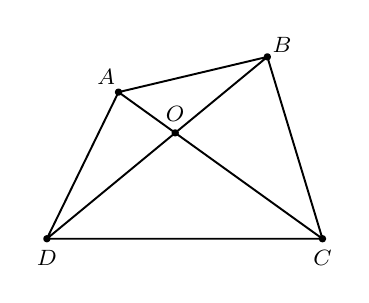
\begin{tikzpicture}[scale=0.7,line width=0.7pt, font=\footnotesize, line join=round, line cap=round, >=stealth]
	%% Khai bao diem		
	\path
	(0,0) coordinate (D)
	(5,0) coordinate (C)
	(1.3,2.66) coordinate (A)
	(4,3.3) coordinate (B)
	(intersection of A--C and B--D) coordinate (O)
	;
	
	\draw (A)--(B)--(C)--(D)--(A)--(C) (B)--(D);
	%% vẽ điểm
	\foreach \x/\g in {A/130,B/40,C/-90,D/-90,O/90}
	\draw[fill=black] (\x) circle (.049)+(\g:.35)
	node{$\x$};	
\end{tikzpicture}
\end{center}
\begin{listEX}[1]
	\item Theo quy tắc ba điểm ta có
	\[\overrightarrow{AB}+\overrightarrow{BC}+\overrightarrow{CD}+\overrightarrow{DA}=\overrightarrow{AC}+\overrightarrow{CD}+\overrightarrow{DA}=\overrightarrow{AD}+\overrightarrow{DA}=\overrightarrow{AA}=\overrightarrow{0}.\]
	\item Theo quy tắc ba điểm ta có
	\[\overrightarrow{AB}+\overrightarrow{CD}+\overrightarrow{BC}=\overrightarrow{AB}+\overrightarrow{BC}+\overrightarrow{CD}=\overrightarrow{AC}+\overrightarrow{CD}=\overrightarrow{AD}.\]
	\item  Theo quy tắc hiệu ta có $\overrightarrow{A B}-\overrightarrow{A D}=\overrightarrow{D B}$.
	\item Theo quy tắc hiệu và quy tắc ba điểm ta có
	\[\overrightarrow{OD}-\overrightarrow{OC}+\overrightarrow{CB}-\overrightarrow{CD}=\overrightarrow{CD}+\overrightarrow{DB}=\overrightarrow{CB}.\]
\end{listEX}
}
\end{ex}

\begin{ex}%[Dự án đề cương 3 Khối NH24-25-Dot1-Bùi Quang Phú]%[0H5C2-1]
Cho tam giác $ABC$ có trung tuyến $AM$. Trên cạnh $AC$ lấy hai điểm $E$, $F$ sao cho $AE=EF=FC$; $BE$ cắt trung tuyến $AM$ tại $N$. Xác định vectơ $\overrightarrow{AE}+\overrightarrow{AF}+\overrightarrow{AN}+\overrightarrow{MN}$.
\loigiai{
\begin{center}
	\begin{tikzpicture}[scale=0.7,line width=0.7pt, font=\footnotesize, line join=round, line cap=round, >=stealth]
		%% Khai bao diem		
	\path
	(0,0) coordinate (B)
	(5,0) coordinate (C)
	(1.3,3) coordinate (A)
	($(A)!1/3!(C)$) coordinate (E)
	($(A)!2/3!(C)$) coordinate (F)
	($(B)!1/2!(C)$) coordinate (M)
	(intersection of A--M and B--E) coordinate (N)
	;
	
	\draw (A)--(B)--(C)--(A)--(M) (B)--(E) (M)--(F);
	%% vẽ điểm
	\foreach \x/\g in {A/90,B/-90,C/-90,E/50,F/50,N/160,M/-90}
	\draw[fill=black] (\x) circle (.049)+(\g:.35)
	node{$\x$};	
	\end{tikzpicture}
\end{center}
Vì $AE=EF=FC$ nên $AF=EC$. Khi đó $\overrightarrow{AF}=\overrightarrow{EC}$.\\
Suy ra $\overrightarrow{AE}+\overrightarrow{AF}=\overrightarrow{AE}+\overrightarrow{EC}=\overrightarrow{AC}$.\\
Vì $MF$ là đường trung bình của $\triangle BEC$ nên $MF \parallel BE$.\\
Vì $\heva{
	& NE \parallel MF~(\text{vì } MF \parallel BE)  \\
	&  E \text { là trung điểm của } A F \\
}$ nên $N$ là trung điểm của $AM$.\\
Suy ra $\overrightarrow{AN}+\overrightarrow{MN}=\overrightarrow{0}$.\\
Vậy $\overrightarrow{AE}+\overrightarrow{AF}+\overrightarrow{AN}+\overrightarrow{MN}=\overrightarrow{AC}$.
}	
\end{ex}

\begin{ex}%[Dự án đề cương 3 Khối NH24-25-Dot1-Bùi Quang Phú]%[0H5V2-2]
Cho tứ giác $ABCD$. Gọi $E$, $F$, $G$, $H$ lần lượt là trung điểm của $AB$, $BC$, $CD$, $DA$ và $M$ là một điểm tùy ý. Chứng minh rằng:
\begin{listEX}[1]
\item $\overrightarrow{AF}+\overrightarrow{BG}+\overrightarrow{CH}+\overrightarrow{DE}=\overrightarrow{0}$.
\item $\overrightarrow{MA}+\overrightarrow{MB}+\overrightarrow{MC}+\overrightarrow{MD}=\overrightarrow{ME}+\overrightarrow{MF}+\overrightarrow{MG}+\overrightarrow{MH}$.	
\end{listEX}
\loigiai{
\begin{center}
	\begin{tikzpicture}[scale=0.7,line width=0.7pt, font=\footnotesize, line join=round, line cap=round, >=stealth]
		%% Khai bao diem		
	\path
	(0,0) coordinate (D)
	(5,0) coordinate (C)
	(1.3,2.66) coordinate (A)
	(4,3.3) coordinate (B)
	($(A)!1/2!(B)$) coordinate (E)
	($(B)!1/2!(C)$) coordinate (F)
	($(C)!1/2!(D)$) coordinate (G)
	($(D)!1/2!(A)$) coordinate (H)
	;
	
	\draw (A)--(B)--(C)--(D)--(A)--(C) (E)--(F)--(G)--(H)--(E);
	%% vẽ điểm
	\foreach \x/\g in {A/130,B/40,C/-90,D/-90,E/90,F/20,G/-90,H/160}
	\draw[fill=black] (\x) circle (.049)+(\g:.35)
	node{$\x$};	
	\end{tikzpicture}
\end{center}
\begin{listEX}[1]
\item Vì $EF$ là đường trung bình của $\triangle ABC$ nên $EF=\dfrac{1}{2} AC$ và $E F \parallel A C$.\\
Vì $HG$ là đường trung bình của $\triangle ADC$ nên $HG=\dfrac{1}{2} AC$ và $HG \parallel AC$.\\[0.2cm]
Suy ra $EF=HG$ và $E F \parallel HG$.\\[0.2cm]
Do đó $\overrightarrow{EF}=\overrightarrow{HG}$ hay $\overrightarrow{EF}+\overrightarrow{GH}=\overrightarrow{0}$.\\[0.2cm]
Ta có	
\[\begin{aligned}
	\overrightarrow{AF}+\overrightarrow{BG}+\overrightarrow{CH}+\overrightarrow{DE} & =\overrightarrow{AE}+\overrightarrow{EF}+\overrightarrow{BE}+\overrightarrow{EG}+\overrightarrow{CG}+\overrightarrow{GH}+\overrightarrow{DG}+\overrightarrow{GE} \\
	& =\left(\overrightarrow{AE}+\overrightarrow{BE}\right)+\left(\overrightarrow{CG}+\overrightarrow{DG}\right)+\left(\overrightarrow{EF}+\overrightarrow{GH}\right)+\left(\overrightarrow{EG}+\overrightarrow{GE}\right) \\
	& =\overrightarrow{0}.
\end{aligned}\]
\item Theo câu a) ta có
\[\begin{aligned}
	& \overrightarrow{AF}+\overrightarrow{BG}+\overrightarrow{CH}+\overrightarrow{DE}=\overrightarrow{0} \\
	\Leftrightarrow~ & \left(\overrightarrow{MF}-\overrightarrow{MA}\right)+\left(\overrightarrow{MG}-\overrightarrow{MB}\right)+\left(\overrightarrow{MH}-\overrightarrow{MC}\right)+\left(\overrightarrow{ME}-\overrightarrow{MD}\right)=\overrightarrow{0} \\
	\Leftrightarrow~ & \overrightarrow{MF}+\overrightarrow{MG}+\overrightarrow{MH}+\overrightarrow{ME}=\overrightarrow{MA}+\overrightarrow{MB}+\overrightarrow{MC}+\overrightarrow{MD} ~~\text {(đpcm)}
\end{aligned}\]
\end{listEX}
}
\end{ex}

\begin{ex}%[Dự án đề cương 3 Khối NH24-25-Dot1-Bùi Quang Phú]%[0H5V2-2]
Cho tam giác $ABC$. Từ các điểm $A$, $B$, $C$ ta dựng các vectơ $\overrightarrow{AA'}=\overrightarrow{BB'}=\overrightarrow{CC'}$. Chứng minh rằng:
\begin{listEX}[1]
\item $\overrightarrow{BB'}+\overrightarrow{CC'}+\overrightarrow{BA}+\overrightarrow{CA}=\overrightarrow{BA'}+\overrightarrow{CA'}$.
\item $\overrightarrow{AA'}+\overrightarrow{BB'}+\overrightarrow{CC'}=\overrightarrow{BA'}+\overrightarrow{CB'}+\overrightarrow{AC'}$.
\end{listEX}
\loigiai{
\begin{center}
	\begin{tikzpicture}[scale=0.7,line width=0.7pt, font=\footnotesize, line join=round, line cap=round, >=stealth]
		%% Khai bao diem		
		\path
		(0,0) coordinate (B)
		(5,0) coordinate (C)
		(1.1,-1.8) coordinate (A)
		($(A)+(1,3.5)$) coordinate (A')
		($(B)+(1,3.5)$) coordinate (B')
		($(C)+(1,3.5)$) coordinate (C')
		;
		
		\draw (A)--(B)--(C)--(A)--(C) (A')--(B')--(C')--(A');
		\draw[thick,-{Stealth[length=2.5mm]}] (A)--(A');
		\draw[thick,-{Stealth[length=2.5mm]}] (B)--(B');
		\draw[thick,-{Stealth[length=2.5mm]}] (C)--(C');
		%% vẽ điểm
		\foreach \x/\g in {A/-90,B/180,C/0,A'/-30,B'/180,C'/0}
		\draw[fill=black] (\x) circle (.049)+(\g:.35)
		node{$\x$};	
	\end{tikzpicture}
\end{center}
\begin{listEX}[1]
	\item Vì $\overrightarrow{AA'}=\overrightarrow{BB'}$ nên $ABB'A'$ là hình bình hành.\\
	 Khi đó $\overrightarrow{BB'}+\overrightarrow{BA}=\overrightarrow{BA'}$.\\
	 Vì $\overrightarrow{AA'}=\overrightarrow{CC'}$ nên $ACC'A'$ là hình bình hành.\\
	 Khi đó $\overrightarrow{CC'}+\overrightarrow{CA}=\overrightarrow{CA'}$.\\
	 Vậy $\overrightarrow{BB'}+\overrightarrow{CC'}+\overrightarrow{BA}+\overrightarrow{CA}=\overrightarrow{BA'}+\overrightarrow{CA'}$.
	\item Ta có
	\[\begin{aligned}
		\overrightarrow{A A'}+\overrightarrow{B B'}+\overrightarrow{C C'} & =\overrightarrow{B A'}-\overrightarrow{B A}+\overrightarrow{C B'}-\overrightarrow{C B}+\overrightarrow{A C'}-\overrightarrow{A C} \\
		& =\overrightarrow{B A'}+\overrightarrow{C B'}+\overrightarrow{A C'}+(\overrightarrow{A B}-\overrightarrow{A C}-\overrightarrow{C B}) \\
		& =\overrightarrow{B A'}+\overrightarrow{C B'}+\overrightarrow{A C'}+(\overrightarrow{C B}-\overrightarrow{C B}) \\
		& =\overrightarrow{B A'}+\overrightarrow{C B'}+\overrightarrow{A C'}~~(\text {đpcm}).
	\end{aligned}\]
\end{listEX}
}
\end{ex}

\begin{ex}%[Dự án đề cương 3 Khối NH24-25-Dot1-Bùi Quang Phú]%[0H5H2-4]
Cho hình vuông $ABCD$ tâm $O$ có cạnh bằng $a$. Tính
\begin{listEX}[3]
\item $\left|\overrightarrow{AB}+\overrightarrow{AD}\right|$;
\item $\left|\overrightarrow{AB}-\overrightarrow{AC}\right|$;
\item $\left|\overrightarrow{OA}+\overrightarrow{OB}\right|$.
\end{listEX}
\loigiai{
\begin{center}
	\begin{tikzpicture}[scale=0.7,line width=0.7pt, font=\footnotesize, line join=round, line cap=round, >=stealth]
		%% Khai bao diem		
		\path
		(0,0) coordinate (D)
		(4,0) coordinate (C)
		(0,4) coordinate (A)
		($(A)+(C)-(D)$) coordinate (B)
		(intersection of A--C and B--D) coordinate (O)
		;
		
		\draw (A)--(B)--(C)--(D)--(A)--(C) (B)--(D);
		%% vẽ điểm
		\foreach \x/\g in {A/90,B/90,C/-90,D/-90,O/90}
		\draw[fill=black] (\x) circle (.049)+(\g:.35)
		node{$\x$};	
	\end{tikzpicture}
\end{center}
\begin{listEX}[1]
	\item $\left|\overrightarrow{AB}+\overrightarrow{AD}\right|=\left|\overrightarrow{AC}\right|=AC$.\\
	Xét $\triangle A B C$ vuông tại $B$ có $AC=\sqrt{A B^{2}+B C^{2}}=\sqrt{a^{2}+a^{2}}=a \sqrt{2}$.\\
	Vậy $\left|\overrightarrow{AB}+\overrightarrow{AD}\right|=a \sqrt{2}$.
	\item $\left|\overrightarrow{AB}-\overrightarrow{AC}\right|=\left|\overrightarrow{CB}\right|=CB=a$.
	\item Vì $O$ là trung điểm của $AC$ nên $\overrightarrow{OA}=\overrightarrow{CO}$.\\
	Ta có $\left|\overrightarrow{OA}+\overrightarrow{OB}\right|=\left|\overrightarrow{CO}+\overrightarrow{OB}\right|=\left|\overrightarrow{CB}\right|=CB=a$.
\end{listEX}
}	
\end{ex}

\begin{ex}%[Dự án đề cương 3 Khối NH24-25-Dot1-Bùi Quang Phú]%[0H5V2-4]
Cho bốn điểm $A$, $B$, $C$, $O$ phân biệt có độ dài ba vectơ $\overrightarrow{OA}$, $\overrightarrow{OB}$, $\overrightarrow{OC}$ cùng bằng $a$ và thỏa mãn $\overrightarrow{OA}+\overrightarrow{OB}+\overrightarrow{OC}=\overrightarrow{0}$.
\begin{listEX}[1]
	\item Tính số đo của $\widehat{AOC}$ và độ dài $\left|\overrightarrow{OA}-\overrightarrow{OC}\right|$.
	\item Tính $\left|\overrightarrow{OB}+\overrightarrow{AC}-\overrightarrow{OA}\right|$.
\end{listEX}
	\loigiai{
\begin{center}
	\begin{tikzpicture}[scale=0.7,line width=0.7pt, font=\footnotesize, line join=round, line cap=round, >=stealth]
		%% Khai bao diem		
	\path
	(0,0) coordinate (O)
	(90:2.5) coordinate (B)
	(210:2.5) coordinate (A)
	(-30:2.5) coordinate (C)
	($(B)+(C)-(A)$) coordinate (D)
	;
	
	\draw (A)--(B)--(C)--(A) (C)--(O)--(B)--(D)--(C) ;
	\draw[thick,-{Stealth[length=2.5mm]}] (A)--(D);
	%% vẽ điểm
	\foreach \x/\g in {A/180,B/90,C/-90,D/90,O/140}
	\draw[fill=black] (\x) circle (.049)+(\g:.35)
	node{$\x$};	
	\end{tikzpicture}
\end{center}
		\begin{listEX}[1]
			\item Ta có ba điểm $A$, $B$, $C$ không thẳng hàng.\\
			Vì $\overrightarrow{OA}+\overrightarrow{OB}+\overrightarrow{OC}=\overrightarrow{0}$ nên $O$ là trọng tâm của $\triangle ABC$.\\
			Mà $OA=OB=OC$, nên $\triangle ABC$ đều.\\
			Khi đó $AO$ là tia phân giác của $\widehat{BAC}$. Suy ra $\widehat{OAC}=30^{\circ}$.\\[0.2cm]
			Xét $\triangle AOC$ cân tại $O$ có $\widehat{AOC}=180^{\circ}-\widehat{OAC}=180^{\circ}-2 \cdot 30^{\circ}=120^{\circ}$.\\
			Áp dụng định lí côsin cho $\triangle A O C$ ta có
			\[AC^{2}=OA^{2}+OC^{2}-2 \cdot OA \cdot OC \cdot \cos \widehat{AOC} \Rightarrow AC=a \sqrt{3}.\]
			Vậy $\left|\overrightarrow{OA}-\overrightarrow{OC}\right|=\left|\overrightarrow{CA}\right|=CA=a\sqrt{3}$.
			\item Dựng $D$ là điểm thứ tư của hình bình hành $B A C D$ và $M$ là trung điểm của $B C$.\\
			Khi đó $AM=\dfrac{AC \sqrt{3}}{2}=\dfrac{3a}{2}$.\\[0.2cm]
			Ví $BACD$ là hình bình hành nên $M$ là trung điểm của $AD$. Suy ra $AD=2AM=3a$.\\[0.2cm]
			Ta có $\left|\overrightarrow{OB}+\overrightarrow{AC}-\overrightarrow{OA}\right|=\left|\overrightarrow{OB}-\overrightarrow{OA}+\overrightarrow{AC}\right|=\left|\overrightarrow{AB}+\overrightarrow{AC}\right|=\left|\overrightarrow{AD}\right|=AD=3a$.
		\end{listEX}
	}	
\end{ex}


\begin{ex}%[Dự án đề cương 3 Khối NH24-25-Dot1-Bùi Quang Phú]%[0H5H2-3]
(\textit{Trích đề thi GKI - THPT Lê Thánh Tông - HCM - Năm học: 2024-2025})\\
	Cho hình bình hành $ABCD$ có tâm $O$.
	\begin{enumerate}
		\item Chứng minh $\overrightarrow{OA} + \overrightarrow{OB} + \overrightarrow{OC} + \overrightarrow{OD} = \overrightarrow{0}$.
		\item Tìm điểm $M$ thỏa mãn $\overrightarrow{MD}-\overrightarrow{CM}+\overrightarrow{OB}=\overrightarrow{AD}+\overrightarrow{OM}$.
	\end{enumerate}
	\loigiai{
		\begin{center}
			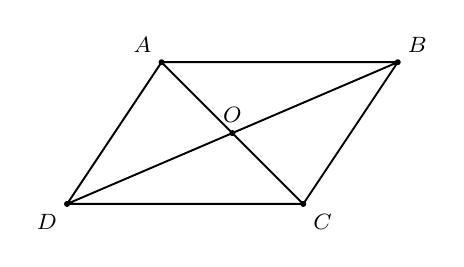
\begin{tikzpicture}[scale=0.6,line width=0.7pt,font=\footnotesize, line join=round, line cap=round, >=stealth]
				\draw[fill=black] (2,3) node[above left]{$A$} coordinate (A) circle(1.2pt);
				\draw[fill=black] (7,3) node[above right]{$B$} coordinate (B) circle(1.2pt);
				\draw[fill=black] (5,0) node[below right]{$C$} coordinate (C) circle(1.2pt);
				\draw[fill=black] (0,0) node[below left]{$D$} coordinate (D) circle(1.2pt);
				\draw[fill=black] (3.5,1.5) node[above]{$O$} coordinate (O) circle(1.2pt);
				\draw (A)--(B)--(C)--(D)--(A) (A)--(C) (B)--(D);
			\end{tikzpicture}
		\end{center}
		\begin{enumerate}
			\item Ta có $O$ là tâm hình bình hành $ABCD$ nên $O$ là trung điểm của $AC$ và $BD$.\\
			Suy ra $\overrightarrow{OA}+ \overrightarrow{OC}=\overrightarrow{0}$ và $\overrightarrow{OB} + \overrightarrow{OD}=\overrightarrow{0}$. \\
			Khi đó $\overrightarrow{OA} + \overrightarrow{OB} + \overrightarrow{OC} + \overrightarrow{OD} = \left(\overrightarrow{OA}+ \overrightarrow{OC} \right) + \left( \overrightarrow{OB} + \overrightarrow{OD} \right) =\overrightarrow{0} + \overrightarrow{0} = \overrightarrow{0}$.
			\item Ta có
			\begin{eqnarray*}
				& &\overrightarrow{MD}-\overrightarrow{CM}+\overrightarrow{OB}=\overrightarrow{AD}+\overrightarrow{OM}\\
				&\Leftrightarrow & \overrightarrow{AD} - \overrightarrow{AM} + \overrightarrow{MC} = \overrightarrow{AD} + \overrightarrow{OM} - \overrightarrow{OB}\\
				&\Leftrightarrow &\overrightarrow{MA} + \overrightarrow{MC} = \overrightarrow{BM}\\
				&\Leftrightarrow &\overrightarrow{MA} + \overrightarrow{MB} + \overrightarrow{MC} = \overrightarrow{0}\\
				&\Leftrightarrow & M \text{ là trọng tâm tam giác } ABC.
			\end{eqnarray*}
			Vậy $M$ là trọng tâm tam giác $ABC$.
		\end{enumerate}
	}
\end{ex}

\begin{ex}%[Dự án đề cương 3 Khối NH24-25-Dot1-Bùi Quang Phú]%[0H5H2-6]
(\textit{Trích đề thi KSCL hè ban Tự nhiên - THPT Chuyên Lê Hồng Phong - Nam Định - Năm học: 2024-2025})\\
Cho ba lực $\overrightarrow{F_1}=\overrightarrow{O A}$, $\overrightarrow{F_2}=\overrightarrow{O B}$ và $\overrightarrow{F_3}=\overrightarrow{O C}$ cùng tác động vào một vật tại điểm $O$ và vật đứng yên. Cho biết cường độ của $\overrightarrow{F_1}$, $\overrightarrow{F_2}$ lần lượt là $60$N và $80$N và $\widehat{AOB}=90^\circ$ (tham khảo hình vẽ). Hỏi cường độ của lực $\overrightarrow{F_3}$ là bao nhiêu Newton?
	\begin{center}
		\begin{tikzpicture}[scale=1,>=stealth, font=\footnotesize, line join=round, line cap=round]
			\path
			(0,0) coordinate (O)
			(0,1.5) coordinate (B)
%			(2.5,-1.5) coordinate (C)
			
			;
			
			\coordinate[label=left:$A$] (A) at (-3,0);
			\coordinate (D) at ($(A)+(B)$);
			\coordinate (C) at ($(O)!2!(D)$);
			\foreach \x/\g in
			{B/0,C/-45,O/-90}
			\fill[black](\x) circle (0.1pt)
			($(\x)+(\g:3mm)$) node{$\x$};
			\draw[->] (O)--(A); \draw[->] (O)--(B);	\draw[->] (O)--(C); 
			\draw (-1,-0.2) node[below] {$\overrightarrow{F_1}$}  (0.1,0.8) node[right] {$\overrightarrow{F_2}$} (1,-1) node {$\overrightarrow{F_3}$}; 
		\end{tikzpicture}
	\end{center}	
	\loigiai{
\begin{center}
	\begin{tikzpicture}[scale=1,>=stealth, font=\footnotesize, line join=round, line cap=round]
		\path
		(0,0) coordinate (O)
		(0,1.5) coordinate (B)
		(2.5,-1.5) coordinate (C)
		
		;
		
		\coordinate[label=left:$A$] (A) at (-3,0);
		\coordinate (D) at ($(A)+(B)$);
		\foreach \x/\g in
		{B/0,C/-45,O/-90,D/90}
		\fill[black](\x) circle (0.1pt)
		($(\x)+(\g:3mm)$) node{$\x$};
		\draw[->] (O)--(A); \draw[->] (O)--(B);	\draw[->] (O)--(C); \draw[->] (O)--(D);
		\draw (-1,-0.2) node[below] {$\overrightarrow{F_1}$}  (0.4,0.8) node[right] {$\overrightarrow{F_2}$} (1,-1) node {$\overrightarrow{F_3}$}; 
	\end{tikzpicture}
\end{center}	
		Để vật đứng yên tại điểm $O$ thì $\overrightarrow{F}_1+\overrightarrow{F}_2+\overrightarrow{F}_3=\overrightarrow{0} \Leftrightarrow \overrightarrow{F}_1+\overrightarrow{F}_2=-\overrightarrow{F}_3$.\\ $\Rightarrow\left|\overrightarrow{F}_3\right|=\left|-\overrightarrow{F}_3\right|=\left|\overrightarrow{F}_1+\overrightarrow{F}_2\right|$.\\
		Ta có $\left|\overrightarrow{F}_1+\overrightarrow{F_2}\right|=|\overrightarrow{O A}+\overrightarrow{O B}|=|\overrightarrow{O D}|=O D$ với $D$ là đỉnh thứ tư của hình bình hành $O B D A$.\\
		Mặt khác, $\widehat{A O B}=90^{\circ}$ nên tứ giác $O B D A$ là hình chữ nhật nên\\
		$O D=\sqrt{O A^2+O B^2}=\sqrt{\left|\overrightarrow{F}_1\right|^2+\left|\overrightarrow{F}_2\right|^2}=100 \Rightarrow\left|\overrightarrow{F}_3\right|=\left|\overrightarrow{F}_1+\overrightarrow{F}_2\right|=100$(N).	
	}
\end{ex}

\begin{ex}%[Dự án đề cương 3 Khối NH24-25-Dot1-Bùi Quang Phú]%[0H5V2-6]
	\immini[thm]{Cho hai lực $\overrightarrow{F}_1=\overrightarrow{OA}$, $\overrightarrow{F}_2=\overrightarrow{OB}$ cùng tác động vào một vật tại điểm $O$. Cường độ hai lực $\overrightarrow{F}_1$, $\overrightarrow{F}_2$ lần lượt là $34$ N và $134$ N. Góc $\widehat{AOB}=120^\circ$. Tính cường độ của lực tổng hợp tác động vào vật. (làm tròn đến hàng đơn vị)}
	{\begin{tikzpicture}[scale=1, font=\footnotesize, line join=round, line cap=round, >=stealth,declare function={a=3; b=5; goc=-60; }]
			\path
			(0,0) coordinate (B)
			(a,0) coordinate (D)
			(goc:b) coordinate (O)
			($(D)+(O)$) coordinate (A);
			\draw (B)--(D)--(A)--(O)--cycle;
			\draw[->=stealth] (O)--(A);
			\draw[->=stealth] (O)--(B);
			\draw[->=stealth] (O)--(D);
			\foreach \x/\y/\z in {A/O/B}{
				\path (\y) pic[draw,angle radius=15pt,right,angle eccentricity=1.2,"$120^\circ$"]{angle = \x--\y--\z};
			}
			\foreach \t/\g in {A/-90,B/90,O/-90,D/90}{
				\fill (\t) circle (1pt) node[shift={(\g:9pt)}]{$ \t $};
			}
	\end{tikzpicture}}
	\loigiai{
		Gọi $\overrightarrow{F}=\overrightarrow{F}_1+ \overrightarrow{F}_2$ là lực tổng hợp cần tìm.\\
		Dựng hình bình hành $OADB$. Ta có $\widehat{OAD}=180^\circ-\widehat{AOB}=60^\circ$.\\
		Khi đó cường độ của lực tổng hợp tác động vào vật là
		\allowdisplaybreaks
		\begin{eqnarray*}
			\left|\overrightarrow{F}\right|=\left|\overrightarrow{OA}+ \overrightarrow{OB}\right|&=&\left|\overrightarrow{OD}\right|\\
			&=&\sqrt{OA^2+AD^2-2\cdot OA\cdot AD\cdot\cos \widehat{OAD}}\\
			&=&\sqrt{34^2+134^2-2\cdot 34\cdot 134\cdot\cos 60^\circ}=2\sqrt{3\,639}\approx 121~ \text{N}.
		\end{eqnarray*}
	}
\end{ex}



\begin{ex}%[Dự án đề cương 3 Khối NH24-25-Dot1-Bùi Quang Phú]%[0H5V2-6]
(\textit{Trích đề thi HKI - THPT Chế Lan Viên - Quảng Trị - Năm học: 2024-2025})\\
Một vật đang ở vị trí $O$ chịu hai lực tác dụng ngược chiều nhau là $\overrightarrow{F}_1$ và $\overrightarrow{F}_2$, trong đó độ lớn lực $\overrightarrow{F}_2$ lớn gấp đôi độ lớn lực $\overrightarrow{F}_1$. Người ta muốn vật dừng lại nên cần tác dụng vào vật hai lực $\overrightarrow{F}_3$, $\overrightarrow{F}_4$ có phương hợp với lực $\overrightarrow{F}_1$ các góc $45^\circ$ như hình vẽ, chúng có độ lớn bằng nhau và bằng $20$\,N. Tìm độ lớn của lực $\overrightarrow{F}_1$ (kết quả làm tròn đến hàng phần mười).
	\begin{center}
		\begin{tikzpicture}[line join=round,line width=0.7pt, line cap=round,>=stealth,font=\footnotesize,scale=0.8]
			\coordinate (O) at (0,0);
			\coordinate (A) at (4,0);
			\coordinate (B) at (-6,0);
			\coordinate (C) at (2,2);
			\coordinate (D) at (2,-2);
			\draw (O) circle (2 cm);
			\draw[->](O)--(A) ;
			\draw[->](O)--(B) ;
			\draw[->,dashed](O)--(C)node [above]{$\overrightarrow{F}_3$} ;
			\draw[->,dashed](O)--(D)node [below]{$\overrightarrow{F}_4$} ;
			\foreach \i/\g in {O/-120}{\draw[fill=black](\i) circle (1.5pt) ($(\i)+(\g:3mm)$) node[scale=1]{$\i$};}
			\path (3.3,0)node [above]{$\overrightarrow{F}_1$};
			\path (-5.5,0)node [above]{$\overrightarrow{F}_2$};
			\pic["$45^\circ$",draw,angle radius=5mm,angle eccentricity=1.6]{angle=A--O--C};
			\pic["$45^\circ$",draw,angle radius=6mm,angle eccentricity=1.5]{angle=D--O--A};
		\end{tikzpicture}
	\end{center}
	\loigiai{
		\immini{Dựng hình bình hành $OACB$ sao cho $OA=OB = 20$, $\widehat{AOC}=\widehat{BOC} = 45^\circ$ và $\overrightarrow{OC}$ cùng hướng với $\overrightarrow{F}_1$.\\
			Đặt $\overrightarrow{OA}=\overrightarrow{F}_3$, $\overrightarrow{OB}=\overrightarrow{F}_4$, $\overrightarrow{OC}=\overrightarrow{F}_1$.\\
			Khi đó $\left|\overrightarrow{F}_3\right|= \left|\overrightarrow{OA}\right| =OA=20$, $\left|\overrightarrow{F}_4\right|= \left| \overrightarrow{OB}\right|=OB=20$, $\overrightarrow{F}_3+\overrightarrow{F}_4=\overrightarrow{F}_{34}=\overrightarrow{OC}$.\\
			Vì $OA = OB$ nên $OACB$  là hình thoi.\\
			Ta có $\widehat{AOB} = \widehat{AOC} + \widehat{COB} = 45^\circ + 45^\circ = 90^\circ$, nên $OACB$  là hình vuông.\\
			Khi đó $OC = \sqrt{2} OA = 20\sqrt{2}\mathrm{\,N}$.\\
			Vì độ lớn lực $\overrightarrow{F}_2$ gấp đôi độ lớn lực $\overrightarrow{F}_1$ và hai lực này ngược chiều, nên 
			$\overrightarrow{F}_2 = -2 \overrightarrow{F}_1$.}
		{
			\begin{tikzpicture}[line join=round, line cap=round,>=stealth,font=\footnotesize,scale=0.8]
				\coordinate (O) at (0,0);
				\coordinate (A) at (2,2);
				\coordinate (B) at (2,-2);
				\coordinate (C) at (4,0);
				\draw[->](O)--(A)--(C)--(B)--cycle (O)--(C) ;	
				\foreach \i/\g in {O/180,A/90,B/-90,C/0}{\draw[fill=black](\i) circle (1.5pt) ($(\i)+(\g:3mm)$) node[scale=1]{$\i$};}
				\pic["$45^\circ$",draw,angle radius=5mm,angle eccentricity=1.6]{angle=C--O--A};
				\pic["$45^\circ$",draw,angle radius=6mm,angle eccentricity=1.5]{angle=B--O--C};
		\end{tikzpicture}}
		\noindent Dưới tác động của $4$ lực, vật ở vị trí cân bằng nên
		\begin{eqnarray*}
			& & \overrightarrow{F}_1 + \overrightarrow{F}_2 + \overrightarrow{F}_3 + \overrightarrow{F}_4 = \overrightarrow{0}\\
			&\Rightarrow& \overrightarrow{F}_1 -2 \overrightarrow{F}_1+\overrightarrow{F}_{34}=\overrightarrow{0}\\
			&\Rightarrow &\overrightarrow{F}_{34}=\overrightarrow{F}_1\\
			&\Rightarrow &\left| \overrightarrow{F}_{1}\right| =\left| \overrightarrow{F}_{34}\right|=OC=20\sqrt{2}\approx 28{,}3\mathrm{\,N}. 
		\end{eqnarray*}
	}
\end{ex}
